\documentclass{gsuthesis}
\graphicspath{{./figures/}}
\usetikzlibrary{decorations,arrows,shapes,positioning}
\tikzset{variable/.default=}
\definecolor{dkgreen}{rgb}{0,0.6,0}
\definecolor{gray}{rgb}{0.5,0.5,0.5}
\definecolor{purple}{rgb}{0.73,0.33,0.83}
\definecolor{aoi}{RGB}{105,210,231}
\definecolor{goldfish}{RGB}{243,134,48}
\definecolor{beachstorm}{RGB}{224,228,204}
\definecolor{pondwater}{RGB}{167,219,216}
\lstdefinestyle{codeblock}{
   language=Matlab,
  morekeywords={break,case,catch,continue,else,elseif,end,for,function,
      global,if,otherwise,persistent,return,switch,try,while,ones,
      squeeze,warning,waitbar,circshift},
   basicstyle=\small\ttfamily,
   keywordstyle=\color{blue},
   commentstyle=\color{dkgreen},
   stringstyle=\color{purple},
   frame=leftline,
   rulecolor=\color{black},
   numbers=left,
   numberstyle=\small,
   stepnumber=1,
   numbersep=13pt,
   backgroundcolor=\color{white},
   tabsize=2,
   showspaces=false,
   showstringspaces=false,
   breaklines=true,
   }
\lstdefinestyle{snippet}{
   language=Matlab,
  morekeywords={break,case,catch,continue,else,elseif,end,for,function,
      global,if,otherwise,persistent,return,switch,try,while,ones,
      squeeze,warning,waitbar,circshift},
   basicstyle=\small\ttfamily,
   keywordstyle=\color{blue},
   commentstyle=\color{dkgreen},
   stringstyle=\color{purple},
   rulecolor=\color{black},
   stepnumber=1,
   numbersep=5pt,
   backgroundcolor=\color{white},
   tabsize=2,
   showspaces=false,
   showstringspaces=false,
   breaklines=true,
   xleftmargin=17pt,
   framexleftmargin=17pt,
   framexrightmargin=5pt,
   framexbottommargin=4pt,
   % frame=bottomline
}
\newenvironment{code}
{\begin{list}{}{\setlength{\leftmargin}{1em}}\item\scriptsize\bfseries}
{\end{list}}
\newcommand{\signhere}{\vspace{0.4in}\rule{\linewidth}{0.5mm}\\}
\newcommand{\degree}{\ensuremath{^\circ}}
\thetitle{Brain tissue temperature dynamics during functional activity and possibilities for optical measurement techniques}
\theauthor{Greggory H. Rothmeier}
\themonth{May}
\theyear{2012}
\thedegree{Master of Science}
\college{College of Arts and Sciences}
\chair{A. G. Unil Perera}
\committee{Mukesh Dhamala,Brian Thoms,D. Michael Crenshaw}
\theabstract{Regional tissue temperature dynamics in the brain is determined by the balance of the metabolic heat production rate and heat exchange with blood flowing through capillaries embedded in the tissue, the surrounding tissues and the environment. Local changes in blood flow and metabolism during functional activity can upset this balance and induce transient temperature changes. Invasive experimental studies in animal models have established that the brain temperature changes during functional activity are observable and a definitive relationship exists between temperature and brain activity. We present a theoretical framework that links tissue temperature dynamics with hemodynamic activity allowing us to non-invasively estimate brain temperature changes from experimentally measured blood-oxygen level dependent (BOLD) signals. With this unified approach, we are able to pinpoint the mechanisms for hemodynamic activity-related temperature increases and decreases.  In addition to this, the potential uses and limitations of optical measurements are discussed.}
\indexwords{Functional magnetic resonance imaging, Blood oxygen level dependent, Temperature, Functional near-infrared spectroscopy}
\dedication{This is dedicated to my parents who made me go to college and to Brooke who inspired me to go to graduate school.  If I wasn't lucky enough to have all of you I would probably be working for Geek Squad.}
\acknowledgments{I want to thank my advisors A. G. Unil Perera and Mukesh Dhamala for their guidance and leadership through my graduate school career.  Likewise, I must thank everyone in Dr. Perera's and Dr. Dhamala's labs for always being helpful over the past couple of years.  Thank you.}
\approvaldate{}
\abbreviations{
  BOLD     & Blood Oxygen Level Dependent          \\
  fMRI     & Functional Magnetic Resonance Imaging \\
  fNIRS    & Functional Near-Infrared Spectroscopy \\
  NMR      & Nuclear Magnetic Resonance            \\
  ROI      & Region of Interest                    \\
  CSF      & Cerebral Spinal Fluid                 \\
  OLM      & Oxygen Limitation Model               \\
  oxyHb   & Oxyhemoglobin                         \\
  deoxyHb & Deoxyhemoglobin                       \\
  TRS      & Time Resolved Spectroscopy            \\
}

\Crefname{figure}{Figure}{Figures} 
\Crefname{equation}{Equation}{Equations} 
\Crefname{table}{Table}{Tables} 
\crefname{figure}{Fig.}{Figs.} 
\crefname{equation}{Eq.}{Eqs.} 
\crefname{table}{Tbl.}{Tbls.} 
\crefrangelabelformat{figure}{(#3#1#4) -~(#5#2#6)} 
\crefrangelabelformat{equation}{(#3#1#4) -~(#5#2#6)}

%%%%%%%%%%%%%%%%%%%%%%%%%%%%%%%%%%%%%%%
%%%%%%%%  BEGIN DOCUMENT  %%%%%%%%%%%%%
%%%%%%%%%%%%%%%%%%%%%%%%%%%%%%%%%%%%%%%
\begin{document}
% Everything is kept in seperate *.tex files.  Use this file to change the orders.
\setcounter{page}{-100}  % fix for hyperref
\makeabstract
\maketitle
\makecopyright
\makeapproval
\pagenumbering{roman}
\setcounter{page}{3}
\makededication
\makeacknowledgments
\clearpage\phantomsection
\tableofcontents
\clearpage\phantomsection
\addcontentsline{toc}{chapter}{List of Tables}
\listoftables
\clearpage\phantomsection
\addcontentsline{toc}{chapter}{List of Figures}
\listoffigures
\listofabbreviations
% \currentpdfbookmark{Signature Page}{link:signaturepage}
% \documentclass[11pt]{report}
\usepackage{setspace}
\doublespacing
\newcommand{\signhere}{\vspace{0.3in}\rule{\linewidth}{0.5mm}\\}
\begin{document}
\thispagestyle{empty}
\centering
  \textsc{Brain tissue temperature dynamics during functional activity and possibilities for optical measurement techniques}\\
  \vspace{0.1in}
  A thesis\\
  presented in Partial Fulfillment of Requirements for the Degree of \\ Master of Science in the College of Arts and Sciences \\
  Georgia State University\\
  2012\\
  by\\
  Greggory Rothmeier\\
  \vspace*{\fill}
  Committee:\\
  \begin{singlespace}
    \signhere
    A. G. Unil Perera, Co-chair\\
    \signhere
    Mukesh Dhamala, Co-chair\\
    \signhere
    Brian Thoms, Member\\
    \signhere
    D. Michael Crenshaw, Member \\
    \vspace{0.1in}
    April 3, 2012\\
    \rule{\linewidth}{0.5mm}
    Date\\
    \signhere
    Richard Miller\\
    Department Chair\\
  \end{singlespace}
\end{document}

%%%%%  Chapters  %%%%%%%%%%%%%%
% List of Chapters in the order they need to appear
\clearpage
\pagenumbering{arabic}
\setcounter{page}{1}
\chapter{Introduction}
\label{ch:introduction}

\begin{figure}[tb]
  \centering
  \vspace{10pt}
  % 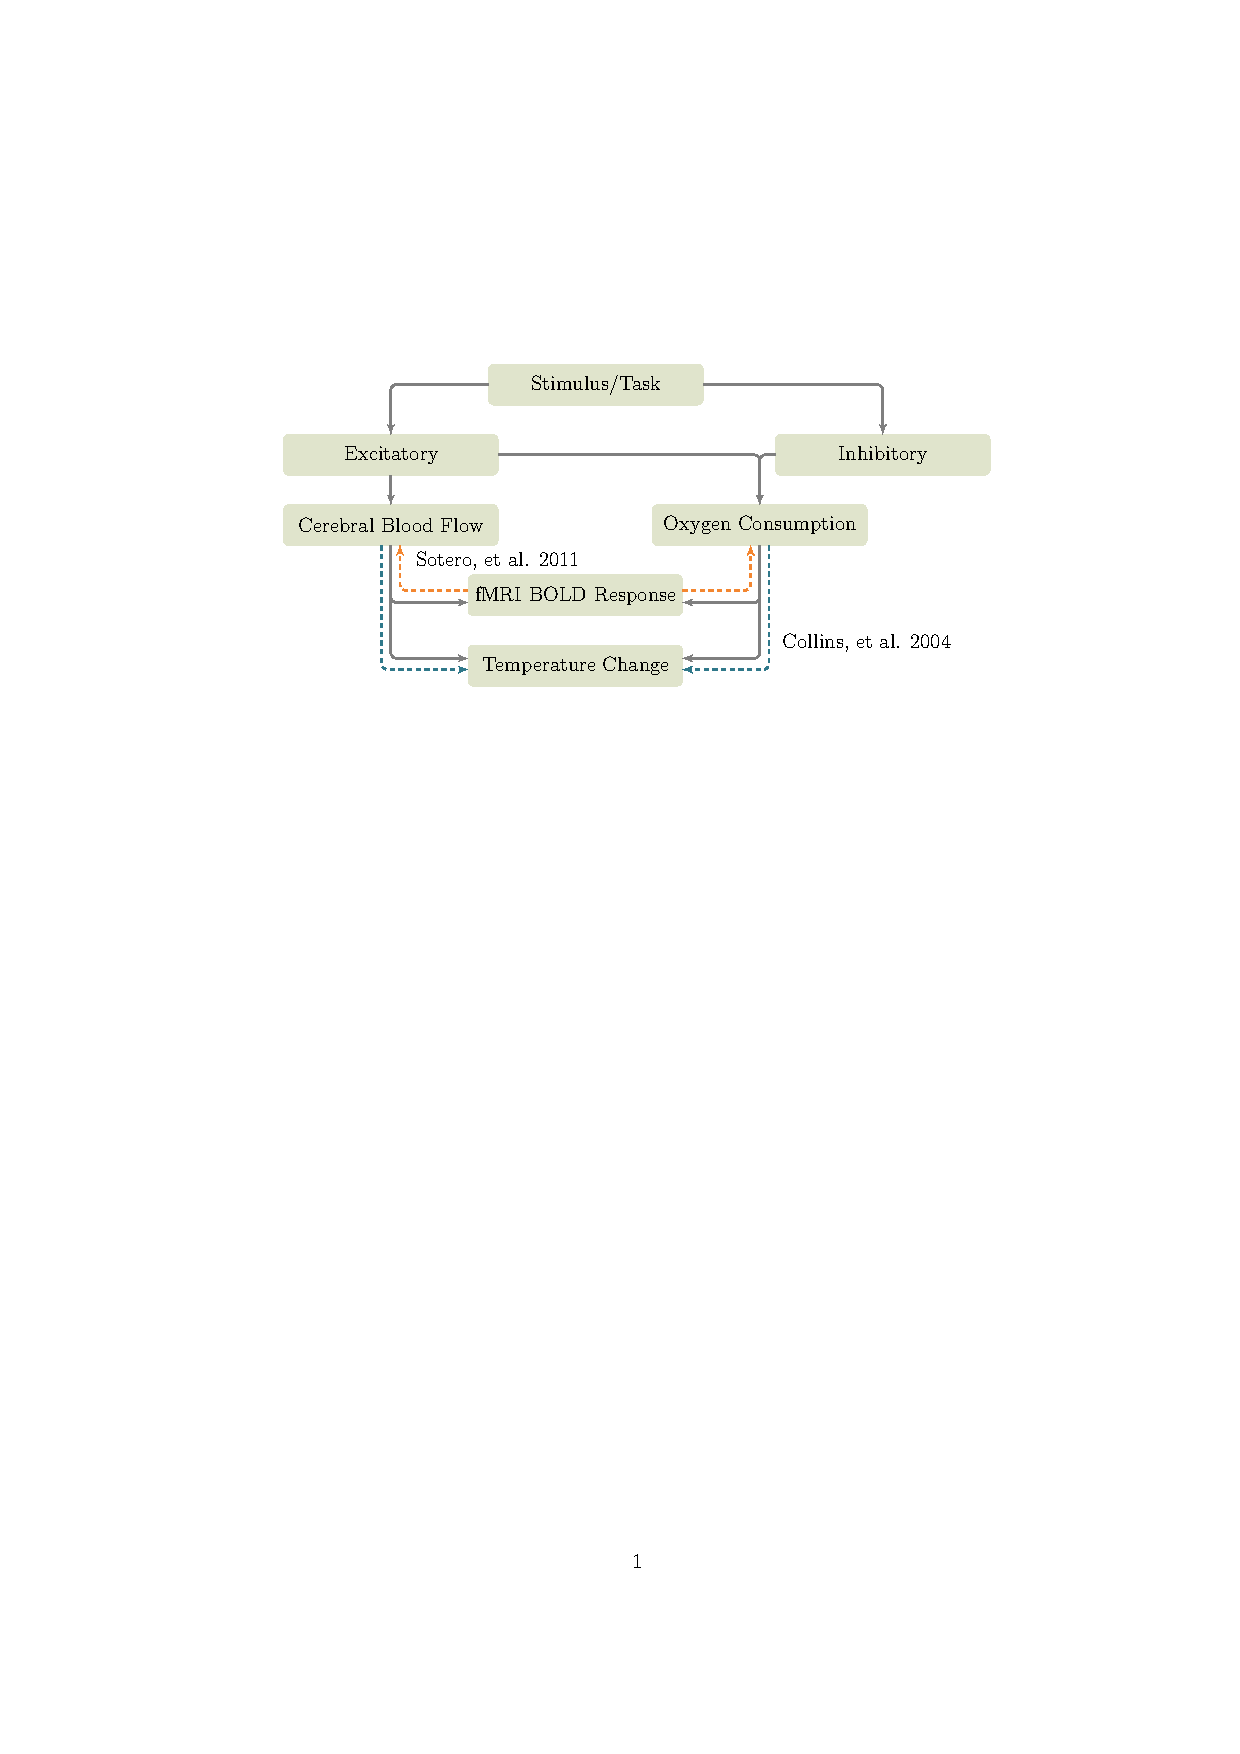
\includegraphics{flowchart}
  \tikzstyle{block} = [draw=none, fill=beachstorm]
\tikzstyle{line} = [draw, very thick, color=black!50, -latex']
\tikzstyle{sotero} = [draw, very thick, dashed, color=goldfish, -latex']
\tikzstyle{collins} = [draw, very thick, dashed, color=aoi, -latex']
\tikzstyle{citation} = [draw=none, fill=white, minimum height=0.5cm, anchor=north, text width=3.5cm]

\begin{tikzpicture}[node distance=0.7cm, rectangle, text width=4.5cm, text badly centered, rounded corners, minimum height=1cm, anchor=north]
  \node[block](stimulus){Stimulus/Task};
  
  \node[block, below=of stimulus, xshift=-5cm](excitatory){Excitatory};
  \node[block, below=of stimulus, xshift= 7cm](inhibitory){Inhibitory};
  
  \node[block, below=of excitatory](cbf){Cerebral Blood Flow};
  \node[block, below=of inhibitory, xshift=-3cm](o2){Oxygen Consumption};
  
  \node[block, below=of cbf, xshift=4.5cm](bold){fMRI BOLD Response};
  \node[block, below=of bold](temp){Temperature Change};
  
  \node[citation](sotero1) at (-3, -4.5) {Sotero, et. al. 2011};
  % \node[citation](sotero1) at (2, -4.5) {Sotero, et. al. 2011};
  % \node[citation](sotero1) at (-4.5, -7.5) {Collins, et. al. 2011};
  \node[citation](sotero1) at (6, -6.5) {Collins, et. al. 2011};
  
  \path[line](stimulus.west) -| (excitatory.north);
  \path[line](stimulus.east) -| (inhibitory.north);
  \path[line](excitatory.south) -- (cbf.north);
  \path[line](excitatory.east) -| (o2.north);
  \path[line](inhibitory.west) -| (o2.north);
  
  \path[line](cbf.south) |- ([yshift=-5pt] bold.west);
  \path[line](cbf.south) |- ([yshift= 5pt] temp.west);
  \path[line](o2.south)  |- ([yshift=-5pt] bold.east);
  \path[line](o2.south)  |- ([yshift= 5pt] temp.east);
  
  \path[sotero]([yshift= 5pt] bold) -| ([xshift= 20pt] cbf);
  \path[sotero]([yshift= 5pt] bold) -| ([xshift=-20pt] o2);
  \path[collins]([xshift=-45pt] cbf) |- ([yshift=-5pt] temp);
  \path[collins]([xshift=45pt] o2)  |- ([yshift= -5pt] temp);
\end{tikzpicture}
  \caption[Generation of the fMRI BOLD response and a corresponding temperature change]{\label{fig:flowchart} Generation of the fMRI BOLD response from changes in neuronal activity.  Black arrows indicate a causal relationship while colored dashed-arrows indicate existing models for the relationship.  The orange line ($\color{goldfish}\bullet$) shows the model proposed by~\citet{sotero2011} to calculate cerebral blood flow and metabolism and the blue line ($\color{aoi}\bullet$) shows how the model proposed by~\citet{collins} is used to calculate temperature.  Modified after~\citet{sotero2007}.}
\end{figure}

Since its invention in the 1950's~\citep{carr1954} and later development in the 1970's~\citep{lauterbur1973}, {M}agnetic {R}esonance {I}maging ({MRI}) has allowed physicians and scientists a detailed view within the human body.  Beginning in the 1990's, it was realized that changes in the local metabolic state affect the local magnetic resonance and provide an indication of brain activity~\citep{ogawa1990,kwong1992}.  This is possible because hemoglobin is diamagnetic in an oxygenated state and paramagnetic when deoxygenated.  Thus as the local concentration of deoxyhemoglobin changes, the local magnetic susceptibility is also altered.  

By combining this affect with the discovery that with an increase in neuronal activity came an increase in local cerebral blood flow (CBF) that far exceeded the increase in cerebral metabolic consumption of oxygen (CMRO$_2$)~\citet{fox1986}, this becomes a powerful tool for measuring brain activity.  The change in local tissue oxygenation found by~\citet{fox1986} is referred to as the blood oxygen dependent~(BOLD) response.  A schematic of the generation of the fMRI BOLD response is provided in~\cref{fig:flowchart}.

A stimulus within a region of the brain induces either an excitatory or inhibitory (or a combination) neuronal response.  An increase in excitatory neuronal activity triggers an increase in CBF which overcompensates for the increase in CMRO$_2$~\citep{fox1986}.  Conversely, an increase in inhibitory neuronal activity does not induce a change in CBF.  An increase in CMRO$_2$ increases the concentration of deoxyhemoglobin (deoxy-Hb) while an increase in CBF delivers more blood to the tissue thereby increasing the concentration of oxyhemoglobin (oxy-Hb).  The change in blood oxygenation is detected by the fMRI as the BOLD response~\citep{kwong1992}.

Along with changes in the BOLD response, changes in CBF and CMRO$_2$ also affect the local tissue temperature.  As glucose is metabolized, heat is released that is primarily dissipated by convection to blood.  Since both BOLD and temperature are dependent on the same factors, it is possible to use the BOLD data collected to calculate the temperature change.  As will be further discussed in~\cref{sec:theoreticalresults}, the resulting temperature change cannot be easily characterized for the entire brain because it's behavior is spatially dependent.

Experimental measurements of activity-induced brain temperature changes are mixed in whether an increase in brain activity increases or decreases local tissue temperature~\citep{mcelligott,kiyatkin,zeschke,george,tachibana}. Current temperature models predict that an increase in activity will result in a decrease in temperature~\citep{sotero2011,yablonskiy,trubel}.  This is generally the prediction because these models generalize the resting-state conditions of the voxel (ignoring spatial dependence) which puts the blood temperature below the resting state tissue temperature.  An increase in blood flow then acts as a coolant for the tissue and lowers the temperature (more on this in~\cref{sec:tempmodelintro}).

I will explore a model which calculates temperature using the fMRI BOLD response for the entire brain, thereby accounting for spatial dependencies.  Additionally, optical measurement techniques including functional near-infrared spectroscopy (fNIRS) and the use of thermal imaging cameras to measure activity-induced brain temperature changes are discussed.
\clearpage\chapter{Calculating Temperature Changes using the fMRI BOLD Response}
    
  \section{\label{sec:tempmodelintro} Introduction}
  Current efforts to model temperature changes be can categorized into two classes.  The first class approaches the problem by considering a single voxel deep within the brain (single-voxel approach) while the second approach considers the brain and head as an entire system (multi-voxel approach).  Each of these methods has their own pros and cons which will be discussed below.
  %%  SINGLE VOXEL APROACH %%
    \subsection{\label{sec:singlevox} Single-Voxel Methods}
    A single-voxel model of temperature was first proposed by SOMEONE, but has been refined over the past HOWLONG years CITEABUNCH to include more terms.  Although different approaches consider different contributions to the temperature change, they all narrow the problem down to a single voxel which is usually 2mm x 2mm x 2mm.  By simplifying the model, the heat equation can be simplified and the calculation is much easier to undertake.  However, since the brain is not homogenous, the values used for parameters such as heat production and thermal conductivity are taken from an average of the tissues.  As a result, this reduces the possible accuracy of such a model when applied to a subject.
    
    The most recently published iteration of a single-voxel model was published by~\citet{sotero2011}.  The basis of this model is a modification of the Penne's Bioheat Equation~\citep{pennes, sotero2011}.
    %%%%%%%  Bio-heat Equation %%%%%%%%%%%%
    \begin{align}
      \label{eq:bioheat}
      C_t \frac{dT(t)}{dt} &= (\Delta H^{\circ}-\Delta H_{b}) CMRO_{2}\mid_{0} m(t) - \rho_{b} C_{b} CBF\mid_{0} f(t) (T(t) - T_{a}) \nonumber \\
      &\qquad {} - \frac{C_{t}}{\tau} (T(t)-T_{0})
    \end{align}
    where $C_t$ is the specific heat of the tissue, $\Delta H^{\circ}$ is the enthalpy released in the oxidation of glucose, $\Delta H_b$ is the enthalpy used to release oxygen from hemoglobin, $COMRO_2 \mid_0$ is the metabolic rate at rest, $\rho_b$ is the blood density, $C_b$ is the specific heat of blood, $CBF\mid_0$ is the cerebral blood flow at rest, $T_a$ is the arterial blood temperature, $C_T$ is the specific heat for the tissue, and $\tau$ is a time constant for conductive heat loss.  The values used are provided in~\cref{tbl:soteroparams}.
    
    One advantage of using~\cref{eq:bioheat} is that the resting state temperature can be analytically determined by substituting $\frac{dT(t)}{dt} = 0$~\citep{sotero2011}.
    %%%%%%%  Resting state temperature %%%%%
    \begin{equation}
      \label{eq:restingtemperature}
      T_{0} = T_{a} + \frac{(\Delta H \mid^{\circ} - \Delta H_{b}) CMRO_{2}\mid_{0}}{\rho_{B} C_{B} CBF\mid_{0}}
    \end{equation}
    If the values provided in~\cref{tbl:soteroparams} are substitued into~\cref{eq:restingtemperature}, a resting temperature of 37.3057\degree C is found.  Since the resting temperature is always greater than the arterial blood temperature, it limits the ability of the model to account for all experimental results. 
    
    While~\cref{eq:bioheat} is appears complicated, conceptually the equation can be easily understood.
    %%%%%%%  Explanation %%%%%%%%%%%%%%%%%%%
    \begin{align}    
      \label{eq:soteroexplaiend}
      change\ in\ temperature\ &=\ heat\ generated\ by\ metabolism\ -\ heat\ lost\ to\ convection\ \nonumber \\
      &\qquad {} -\ heat\ lost\ to\ conduction
    \end{align}
    The system is a balance between heat generation (metabolism) and heat transfer (conduction and convection).  The direction of heat transfer by convection is determined by the difference between the voxel temperature and the arterial blood temperature ($T(t) - T_a$).  Similarly, the direction of heat transfer by conduction is determined by the difference between the voxel temperature and the temperature of the surrounding tissue ($T(t) - T_0$).  Since $T_a$ is less than $T(0)$, an increase in blood flow ($f(t)$) will remove heat from the voxel thereby decreasing the temperature.  Conversely, an increase in metabolism ($m(t)$) without a corresponding change in blood flow, will result in tissue warming.  
    
    %%  MULTI VOXEL APPROACH  %%
    \subsection{\label{sec:multivox} Multi-Voxel Methods}
    The multi-voxel approach to calculating brain tissue temperature alleviates many of the issues that a single-voxel approach has.  The most prominent advantage a multi-voxel approach has is the a result of it accounting for a voxels location relative to the surface of the head and other voxels.  By accounting for a voxel's location, the same BOLD response in two different locations can have vastly different effects on the local tissue temperature (more on this in~\cref{sec:theoreticalresults}).
    At the heart of our method is a three-dimensional implementation of the Pennes bioheat equation (\cref{eq:3dbioheat})\citep{collins}.
    \begin{equation} \label{eq:3dbioheat} 
    	\rho c \frac{dT}{dt} = k \nabla^{2}T-\rho_{blood}f(t)wc_{blood}(T-T_{blood})+m(t)Q_{m} 
    \end{equation}
  where $\rho$ is the tissue density, $c$ is the specific heat of the voxel, $k$ is the thermal conductivity, $\rho_{blood}$ is the blood density, $w$ is perfusion by blood, $c_{blood}$ is the specific heat of blood, $T_{blood}$ is the arterial blood temperature, and $Q_{m}$ is the baseline metabolic heat production. $f(t)$ and $m(t)$ are the time-dependent changes in blood flow and metabolism. These two factors determine the short-term change in temperature and are calculated from the fMRI BOLD response; however what makes this approach more complete than a single-voxel approach is that the relatively slow conductive heat loss makes for a different equilibrium temperature at each voxel.  This affect can only be captured by considering the entire head.  The approach we use is a multi-voxel approach, so more details about this model are discussed in~\cref{sec:approach}.

% THE APPROACH
\section{\label{sec:approach} Our Approach}
\begin{figure}[tb]
  \vspace{10pt}
  \centering
  \tikzstyle{data} = [draw=none, fill=goldfish]
\tikzstyle{temptools} = [draw=none, fill=aoi]
\tikzstyle{spm} = [draw=none, fill=beachstorm]
\tikzstyle{params} = [draw=none, fill=pondwater]
\tikzstyle{line} = [draw, very thick, color=black!50, -latex']

\begin{tikzpicture}[node distance=0.7cm, rectangle, text width=4.5cm, text badly centered, rounded corners, minimum height=1cm, anchor=north]     
  % Left column
    \node[data](fmridata){fMRI BOLD Data};
    \node[temptools, below=of fmridata](calcrest){Calculate resting state (avg\_NII\_rest)};
    \node[temptools, below=of calcrest](normalize){Normalize the data to resting state (avg\_NII\_normalize)};
    \node[temptools, below=of normalize](boldtomf){Calculate the change in metabolism and blood flow (BOLDtoMF)\\Details given in \cref{sec:calcmf}};
    % middle column
    \node[data, right=of fmridata](t1contrast){T1 contrast image};
    \node[spm, below=of t1contrast](segment){Segment image (SPM8)};
    \node[temptools, right=of boldtomf](buildhead){Build head matrix (ImportSegmentedT1)\\Details given in \cref{sec:prephead}};
    % right column
    \node[temptools, right=of buildhead](calcequil){Calculate equilibrium temperature (tempCalcEquilibrium)\\Details given in \cref{sec:calcequilT}};
    \node[params, above=of calcequil, xshift=-2cm](tissueparams){Tissue-specific parameters (given in \cref{tbl:tissues})};
    % bottom
    \node[temptools, below=of buildhead, text width=8cm](calctemp){Find temperature change during activity (tempCalcDynMF)\\Details given in \cref{sec:calcT}};
  
  \path[line](fmridata) -- (calcrest);
  \path[line](calcrest) -- (normalize);
  \path[line](normalize) -- (boldtomf);
  \path[line](t1contrast) -- (segment);
  \path[line](segment) -- (buildhead);
  \path[line](buildhead) -- (calcequil);
  \path[line](boldtomf) |- (calctemp);
  \path[line](buildhead) -- (calctemp);
  \path[line](calcequil) |- (calctemp); 
  \path[line](tissueparams) -| (buildhead);
\end{tikzpicture}
  \caption[Procedure used to calculate temperature change]{\label{fig:procedureflowchart} The procedure used to calculate temperature from BOLD data.  Orange blocks ($\color{goldfish}\bullet$) represent data, the sandy-colored block ($\color{beachstorm}\bullet$) is a step done using SPM8 and the teal blocks ($\color{aoi}\bullet$) are steps done using a function provided within temptools (\cref{apdx:code}).  The name of the function used is in parentheses.}
\end{figure}

  Our approach combines a multi-voxel model (\cref{sec:multivox}) with a model for calculating the change in metabolism and blood flow from the BOLD response.  The Pennes bioheat equation (\cref{eq:bioheat}) \citep{pennes,sotero2011} includes three terms. The first and second terms describe heat generation by metabolism and heat exchange by convection to blood flow.  On shorter time scales, these two terms dominate and are sufficient for determining the temperature change; however, the third term becomes important on longer time scales, so it becomes important in determining the resting-state temperature.
  
  The third term describes the heat exchanged by conduction to surrounding tissues.  This is a comparatively slow process, but on larger time scales, conduction plays an important role in determining the resting state temperature.  When calculating the temperature change, it is important to first have an accurate resting state temperature.  By considering the entire head, out model is able to accurately determine a resting state temperature for each voxel, enabling far more accurate temperature calculations than what is capable with single-voxel approaches.  
  
  \Cref{fig:procedureflowchart} gives a schematic of the temperature calculation procedure.  The orange blocks represent the required data.  The first thing to be done is establish the resting-state temperature for each voxel within the head.  The details of this procedure are given in~\cref{sec:calcequilT}, but in summary a T1 contrast image is segmented using SPM8~(\cref{fig:segmented}) and is combined with tissue-specific parameters~(\cref{tbl:tissues}).  The resulting dataset is then used to determine the resting-state temperature. 
  
  The resting-state time slices from the fMRI BOLD dataset are averaged to create a resting state representative slice.  The rest of the BOLD data is then normalized to this in order to have the normalized change in BOLD response ($\frac{\Delta S}{S_0}$ in~\cref{eq:y}).  This can then be used with~\cref{eq:m,eq:f,eq:y} to create a time series for the change in blood flow and metabolism.  More details about this procedure are given in~\cref{sec:calcmf}.
  
  The following sections provide a detailed explanation of the theory behind our modeling approach.  The code used to implement this procedure is provided and documented in~\cref{apdx:code}.  
  
  % SETUP AND FILE PROCESSING
    \subsection{\label{sec:prephead} Preparing the model of the head}
    \begin{figure}[p] 
      \centering\hspace*{20px} 
    	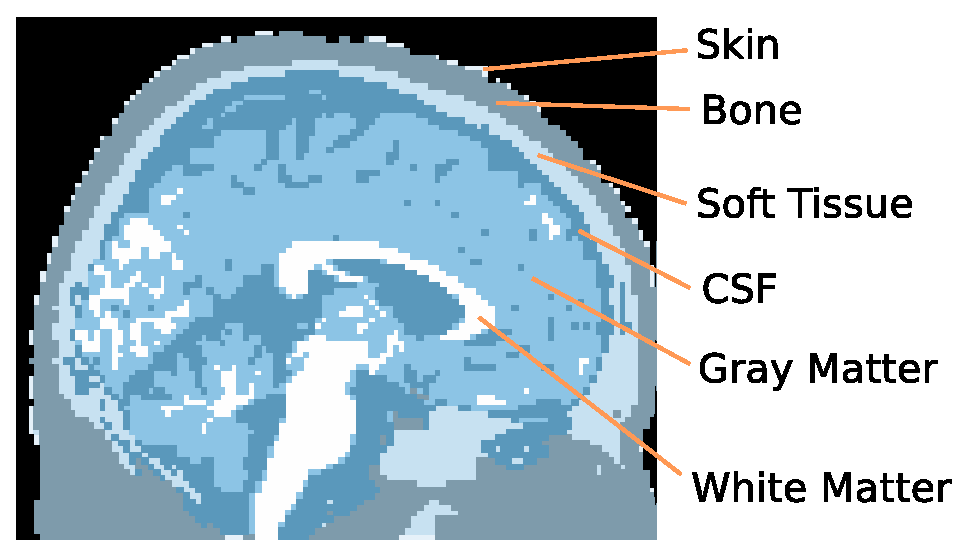
\includegraphics{segmented-head} 
    	\caption[Slice of the segmented head]{\label{fig:segmented} Slice of the segmented head. Each color represents a different tissue type.} 
    \end{figure}
    \begin{table*}[p] 
    		\begin{tabular*}{\linewidth}{@{} l p{2.7cm}p{2cm}p{2.4cm}p{2.5cm}p{2cm}@{}}
    		  \toprule
    		  Tissue & $f_0$ \newline $100 \; ml/(g \; min)$ & $\rho$ \newline $kg/m^{3}$ & $c$ \newline $J \: kg^{-1} \: \degree C^{-1}$ & $k$ \newline $W \: m^{-1} \: \degree C^{-1}$ & $Q_{m}$ \newline $W/m^{3}$ \\
    		  \midrule
    			Bone & 3 & 1,080 & 2,110 & 0.65 & 26.1 \\
    			Cerebrospinal Fluid & 0 & 1,007 & 3,800 & 0.50 & 0 \\
    			Gray Matter & 67.1 & 1,035.5 & 3,680 & 0.565 & 15,575 \\
    			White Matter & 23.7 & 1,027.4 & 3,600 & 0.503 & 5,192 \\
    			Muscle & 3.8 & 1,041 & 3,720 & 0.4975 & 687 \\
    			Skin & 12 & 1,100 & 3,150 & 0.342 & 1,100 \\
    			\bottomrule
    		\end{tabular*}
    		\caption[Tissue-specific parameters]{\label{tbl:tissues} Tissue-specific parameters used to calculate the temperature change (from~\citet{collins}).} 
    \end{table*}
  In order to begin the temperature calculating procedure, a model of the head must first be created.  Using SPM8 (\url{http://www.fil.ion.ucl.ac.uk/spm/}), we segmented a T1 contrast image of the head into five different tissue types: bone, cerebral spinal fluid, gray matter, white matter and soft tissue.  It was assumed that soft tissue voxels that are in contact with air are more appropriately labeled as skin, so in total we are left with a model of the head separated in to six tissue types (\cref{fig:segmented}).  The advantage this has is that we are able to use tissue specific parameters when doing the calculations, thereby improving the accuracy of the results.  The parameters used are available in~\cref{tbl:tissues}.  The code used to create the head matrix is discussed in~\cref{apdx:headmatrix}.

  
  % CALC EQUIL T
    \subsection{\label{sec:calcequilT} Calculating the equilibrium temperature}
  The first step in calculating the temperature change is to first know what the resting state temperature is for each voxel within the head. Our approach was to have the initial temperature for all tissue voxels to be equal to 37\degree C and air voxels are kept at 24\degree C.  The starting temperature of the tissue doesn't affect the final resting state temperature; however, starting off at drastically different values could greatly increase the calculating time required before the temperature stabilizes. The finite difference implementation of the Pennes bioheat equation (\cref{eq:3dbioheat}) is used to update the temperature.  The temperature is updated until the temperature for every voxel has stabilized ($\frac{dT}{dt} < 10^{-6}$ \degree C/s).  Since temperature changes due to changes in neuronal activity are typically greater than $10^{-2}$ \degree C, a change in temperature less than $10^{-6}$ \degree C/s is sufficiently small that transient temperature changes are negligible and temperature can be considered stabilized.  The code used to calculate the equilibrium temperature is detailed in~\cref{apdx:findequil}.
  
  % CALC M AND F
    \subsection{\label{sec:calcmf} Calculating Metabolism and Blood Flow Changes from fMRI BOLD}
    %%%%  Table of values used in Sotero, 2011  %%%%%
    \begin{table*}[p]
      \caption[Parameters used in the single-voxel approximation]{\label{tbl:soteroparams} Parameters used to solve the single-voxel Penne's Bioheat Equation.  (modified from~\citet{sotero2011})}
        \begin{tabular*}{\linewidth}{lp{8.5cm}p{7cm}}
          \toprule
          Parameter & Meaning & Value \\
          \midrule
          T$_{a}$ & Arterial blood temperature & 37\degree C \\
          $C_{tissue}$ & Tissue Heat Capacity & 3.664 J/(gK) \\
          $\Delta H^{\circ}$ & Enthalpy released by oxidation of glucose & $4.7 10^{5}$ J \\
          $\Delta H_{b}$ & Enthalpy used to release O$_{2}$ from hemoglobin & $2.8 10^{4}$ J \\
          CMRO$_{2}\mid_{0}$ & Cerebral metabolic rate of O$_{2}$ consumption at rest & $0.0263 10^{-6}$ mol/(gs) \\
          CBF$\mid_{0}$ & Cerebral blood flow at rest & 0.0093 cm\textsuperscript{3}/(gs) \\
          $\rho_{b}$ & Blood density & 1.05 g/cm\textsuperscript{3} \\
          C$_{B}$ & Blood heat capacity & 3.894 J/(gK) \\
          $\tau$ & Time constant for conductive heat loss from the ROI to the surrounding tissue & 190.52 s \\
          a, b, c & Parameters of the gamma function fitted from E(f) vs. f & 0.4492, 0.2216, $-0.9872$ \\
          A & Maximum BOLD signal change & 0.22 \\
          $\alpha$ & Steady state flow-volume relation & 0.4 \\
          $\beta$ & Field-strength dependent parameter & 1.5 \\
          \midrule
          Variable & Meaning & \\
          \midrule
          m(t) & CMRO$_2$ normalized to baseline & \\
          f(t) & CBF normalized to baseline & \\
          T(t) & Temperature & \\
          W(t) & Lambert W Function & \\
          $\frac{\Delta S(t)}{S_0}$ & Change in BOLD signal normalized to rest & \\
          \bottomrule
        \end{tabular*}
    \end{table*}
    This is the critical step where we use fMRI BOLD data to calculate the normalized change in metabolism and blood flow.  The method used~\citep{sotero2011} is an assemblage of a couple other works~\citep{buxton2004,buxton1997,fox1988,leithner2009,lin2010,davis1998}. It starts by using the relation between metabolism and blood flow proposed by~\citet{buxton2004}:
    \begin{equation} \label{eq:mf}
      m(t)=f(t)\frac{E(t)}{E_0}
    \end{equation}
  where $E_0$ is the oxygen extraction at rest and $E(f)$ is
    \begin{equation} \label{eq:E}
      E(f)=1-(1-E_0)^{\frac{1}{f(t)}}
    \end{equation}
  in accordance with the oxygen limitation model~\citep{buxton1997}.  Combining~\cref{eq:mf} with~\cref{eq:E} yields
    \begin{equation} \label{eq:EmfCombined}
      m(t)=\frac{f(t)}{E_0}\left[1-(1-E_0)^{\frac{1}{f(t)}}\right]
    \end{equation}
  \Citet{sotero2011} goes about solving~\cref{eq:EmfCombined} by adjusting $E(t)$ data generated by~\cref{eq:E} and fitting it to the gamma function for the $f$ range (0.7--2.0) that is within experimentally reported values~\citep{fox1988,leithner2009,lin2010}:
    \begin{equation} \label{eq:gammafct}
      \frac{E(f)}{E_0}=af^{c}(t)e^{-bf(t)}
    \end{equation}
  where values for a, b and c are provided in~\cref{tbl:soteroparams}.  From this approximation we have the final form of metabolism:
    \begin{equation} \label{eq:m} 
      m(t)=af^{c+1}(t)e^{-bf(t)}.
    \end{equation}
  As proposed by~\citet{davis1998}, the BOLD signal changes ($\frac{\Delta S(t)}{S_0}$) can be described in terms of $m(t)$ and $f(t)$:
    \begin{equation} \label{eq:S}
      \frac{\Delta S(t)}{S_0} = \frac{S(t)-S_0}{S_0} = A(1-f^{\alpha-\beta}(t) m^\beta(t))
    \end{equation}
  Substituting~\cref{eq:m} into~\cref{eq:S} yields
    \begin{equation} \label{eq:mAndS}
      f(t)e^{-\frac{b \beta}{\alpha + \beta c}f(t)}=\left(\frac{\left(A-\frac{\Delta S(t)}{S_0}\right)}{A a^\beta}\right)^{\frac{1}{\alpha+\beta c}}
    \end{equation}
  where A is the maximum change in BOLD signal.  Multiplying each side by $-\frac{b\beta}{\alpha+\beta c}$ gives
    \begin{equation} \label{eq:mAndSmultiplied}
      -\frac{b\beta}{\alpha+\beta c} f(t)e^{-\frac{b \beta}{\alpha + \beta c}f(t)}=-\frac{b\beta}{\alpha+\beta c} \left(\frac{\left(A-\frac{\Delta S(t)}{S_0}\right)}{A a^\beta}\right)^{\frac{1}{\alpha+\beta c}}
    \end{equation}
  which can be solved by using the Lambert W function
    \begin{equation} \label{eq:lambertW}
      z=W(x)
    \end{equation}
  where z is given by
    \begin{equation} \label{eq:lambertWsetup}
      z e^z = x
    \end{equation}
  Finally, $f(t)$ is obtained from~\cref{eq:mAndSmultiplied}
    \begin{equation} \label{eq:f}
      f(t)=\frac{\alpha+\beta c}{b \beta}W(y(t))
    \end{equation}
  where
    \begin{equation} \label{eq:y} 
    	y(t)=-\frac{b \beta}{\alpha+\beta c} \left[\frac{(A-\frac{S(t)}{S_{0}}-1)}{A a^{\beta}}\right]^{\left(\frac{1}{\alpha+\beta c}\right)} 
    \end{equation}
  is a function of the BOLD signal.  Using \cref{eq:m,eq:f,eq:y} allows for the metabolism and blood flow to be calculated from the BOLD signal (values used are provided in~\cref{tbl:soteroparams}).
  
    In order to process the files, the BOLD dataset is stored in folder as a separate NIFTI (*.nii) file for each time step.  The first step in processing the data for temperature calculations is to determine a resting state BOLD signal ($S_0$).  The resting state is calculated by taking the voxel-wise mean of the data when the subject is at rest (i.e. the first and last 20 seconds).  This results in one data set where each voxel is a mean of all of the voxels at the location over time ($S_0$).  In order to calculate the metabolism and blood flow, the BOLD dataset needs to be normalized to this resting state ($\frac{\Delta S(t)}{S_0}$).  
    
    Once $\frac{\Delta S(t)}{S_0}$ is known for each time step, \cref{eq:m,eq:f,eq:y} can be used to calculate the metabolism and blood flow. The implementation of this procedure is discussed in~\cref{apdx:fmriprocessing}. 

  % CALC CHANGE IN T
    \subsection{\label{sec:calcT} Calculating the change in temperature in the active brain}
    As discussed in~\cref{sec:multivox}, the foundation of the model is the Penne's bioheat equation,~\cref{eq:3dbioheat}.  The metabolism and blood flow time-courses calculated in~\cref{sec:calcmf} are used to scale the baseline heat production and blood profusion.  This, in turn, induces a change in the temperature.
    
    The Penne's bioheat equation (\cref{eq:3dbioheat}) is implemented using the finite difference method:
    \begin{equation}
      \label{eq:finitedifference}
      \dot{T}(t) \approx \frac{T(t+l)-T(t)}{l}
    \end{equation}
    where $T(t)$ is the temperature at time $t$ and $l$ is the time step size. Next, we can also approximate $\nabla^{2} T$ by using the finite difference method
    \begin{align}
      \frac{\partial^2T(t;x,y,z)}{\partial x^2} &\approx \frac{T(t;x+h,y,z)-2 T(t;x,y,z)+T(t;x-h,y,z)}{h^2} \notag\\
      \frac{\partial^2T(t;x,y,z)}{\partial y^2} &\approx \frac{T(t;x,y+h,z)-2 T(t;x,y,z)+T(t;x,y-h,z)}{h^2} \notag\\
      \frac{\partial^2T(t;x,y,z)}{\partial z^2} &\approx \frac{T(t;x,y,z+h)-2 T(t;x,y,z)+T(t;x,y,z-h)}{h^2}\label{eq:fdspatial}
    \end{align}
where 
  \begin{equation}
    \label{eq:leplaceT}
    \nabla^{2} T = 
    \frac{\partial^2T(t;x,y,z)}{\partial x^2} + 
    \frac{\partial^2T(t;x,y,z)}{\partial y^2} + 
    \frac{\partial^2T(t;x,y,z)}{\partial z^2}
  \end{equation}
\Cref{eq:leplaceT} can be subtitued into the Penne's bioheat equation~(\cref{eq:3dbioheat})
  \begin{equation}
    \rho c \dot{T} = k_x \frac{\partial^2 T}{\partial x^2} + k_y \frac{\partial^2 T}{\partial y^2} + k_z \frac{\partial^2 T}{\partial z^2} -\rho_{blood}f(t)wc_{blood}(T-T_{blood})+m(t)Q_{m} \label{eq:simplifiedbioheat}
  \end{equation}
  where $\dot{T}$ is the first-derivative of temperature with respect to time, $k_x$ is the thermal conductivity in the x-direction, $k_y$ is the thermal conductivity in the y-direction and $k_z$ is the thermal conductivity in the z-direction.
  Substituting~\cref{eq:fdspatial,eq:finitedifference} into~\cref{eq:simplifiedbioheat} yields
  \begin{align}
    \rho c \frac{T(t+l;x,y,z)-T(t;x,y,z)}{l} \approx \frac{1}{h^2} 
    & [k_x (T(t;x+h,y,z)-2 T(t;x,y,z)+T(t;x-h,y,z)) \notag\\
    & + k_y (T(t;x,y+h,z)-2 T(t;x,y,z)+T(t;x,y-h,z))\notag\\
    & + k_z (T(t;x,y,z+h)-2 T(t;x,y,z)+T(t;x,y,z-h))]\notag\\
    & -\rho_{blood}f(t)wc_{blood}(T-T_{blood})+m(t)Q_{m}
  \end{align}
  which is then rearranged to solve for $T(t+l;x,y,z)$
  \begin{align}
    \label{eq:fdfinal}
    T(t+l;x,y,z) \approx T(t;x,y,z) + \frac{l}{\rho c h^2} 
    & [k_x (T(t;x+h,y,z)-2 T(t;x,y,z)+T(t;x-h,y,z)) \notag\\
    & + k_y (T(t;x,y+h,z)-2 T(t;x,y,z)+T(t;x,y-h,z))\notag\\
    & + k_z (T(t;x,y,z+h)-2 T(t;x,y,z)+T(t;x,y,z-h))]\notag\\
    & -\rho_{blood}f(t)wc_{blood}(T-T_{blood})+m(t)Q_{m}
  \end{align}
  The time step size (l) can be picked arbitrarily, however the spatial step size (h) is limited to the voxel spacing.
  
  The final equation~(\cref{eq:fdfinal}) gives a method for calculating the next time step ($T(t+l)$) from the current time step ($T(t)$).  The implementation of this equation is discussed in~\cref{apdx:tempCalcDynMF}.
  
% RESULTS
  \section{\label{sec:results} Results} 
   In order to understand the behavior of the model, we first applied it simulated BOLD data that was generated by convolving a boxcar function with the hemodynamic response function provided by SPM8.  After we understood the behavior of the model, we then applied it to experimental BOLD data that was collected by~\citet{dhamala}.

  %% THEORETICAL RESULTS %%
    \subsection{\label{sec:theoreticalresults} Using Theoretical BOLD Data}
    \FloatBarrier
    \begin{figure}[p] 
    	\begin{center}
    		\begin{tabularx}{\textwidth}{cc}
    			\raisebox{20px}{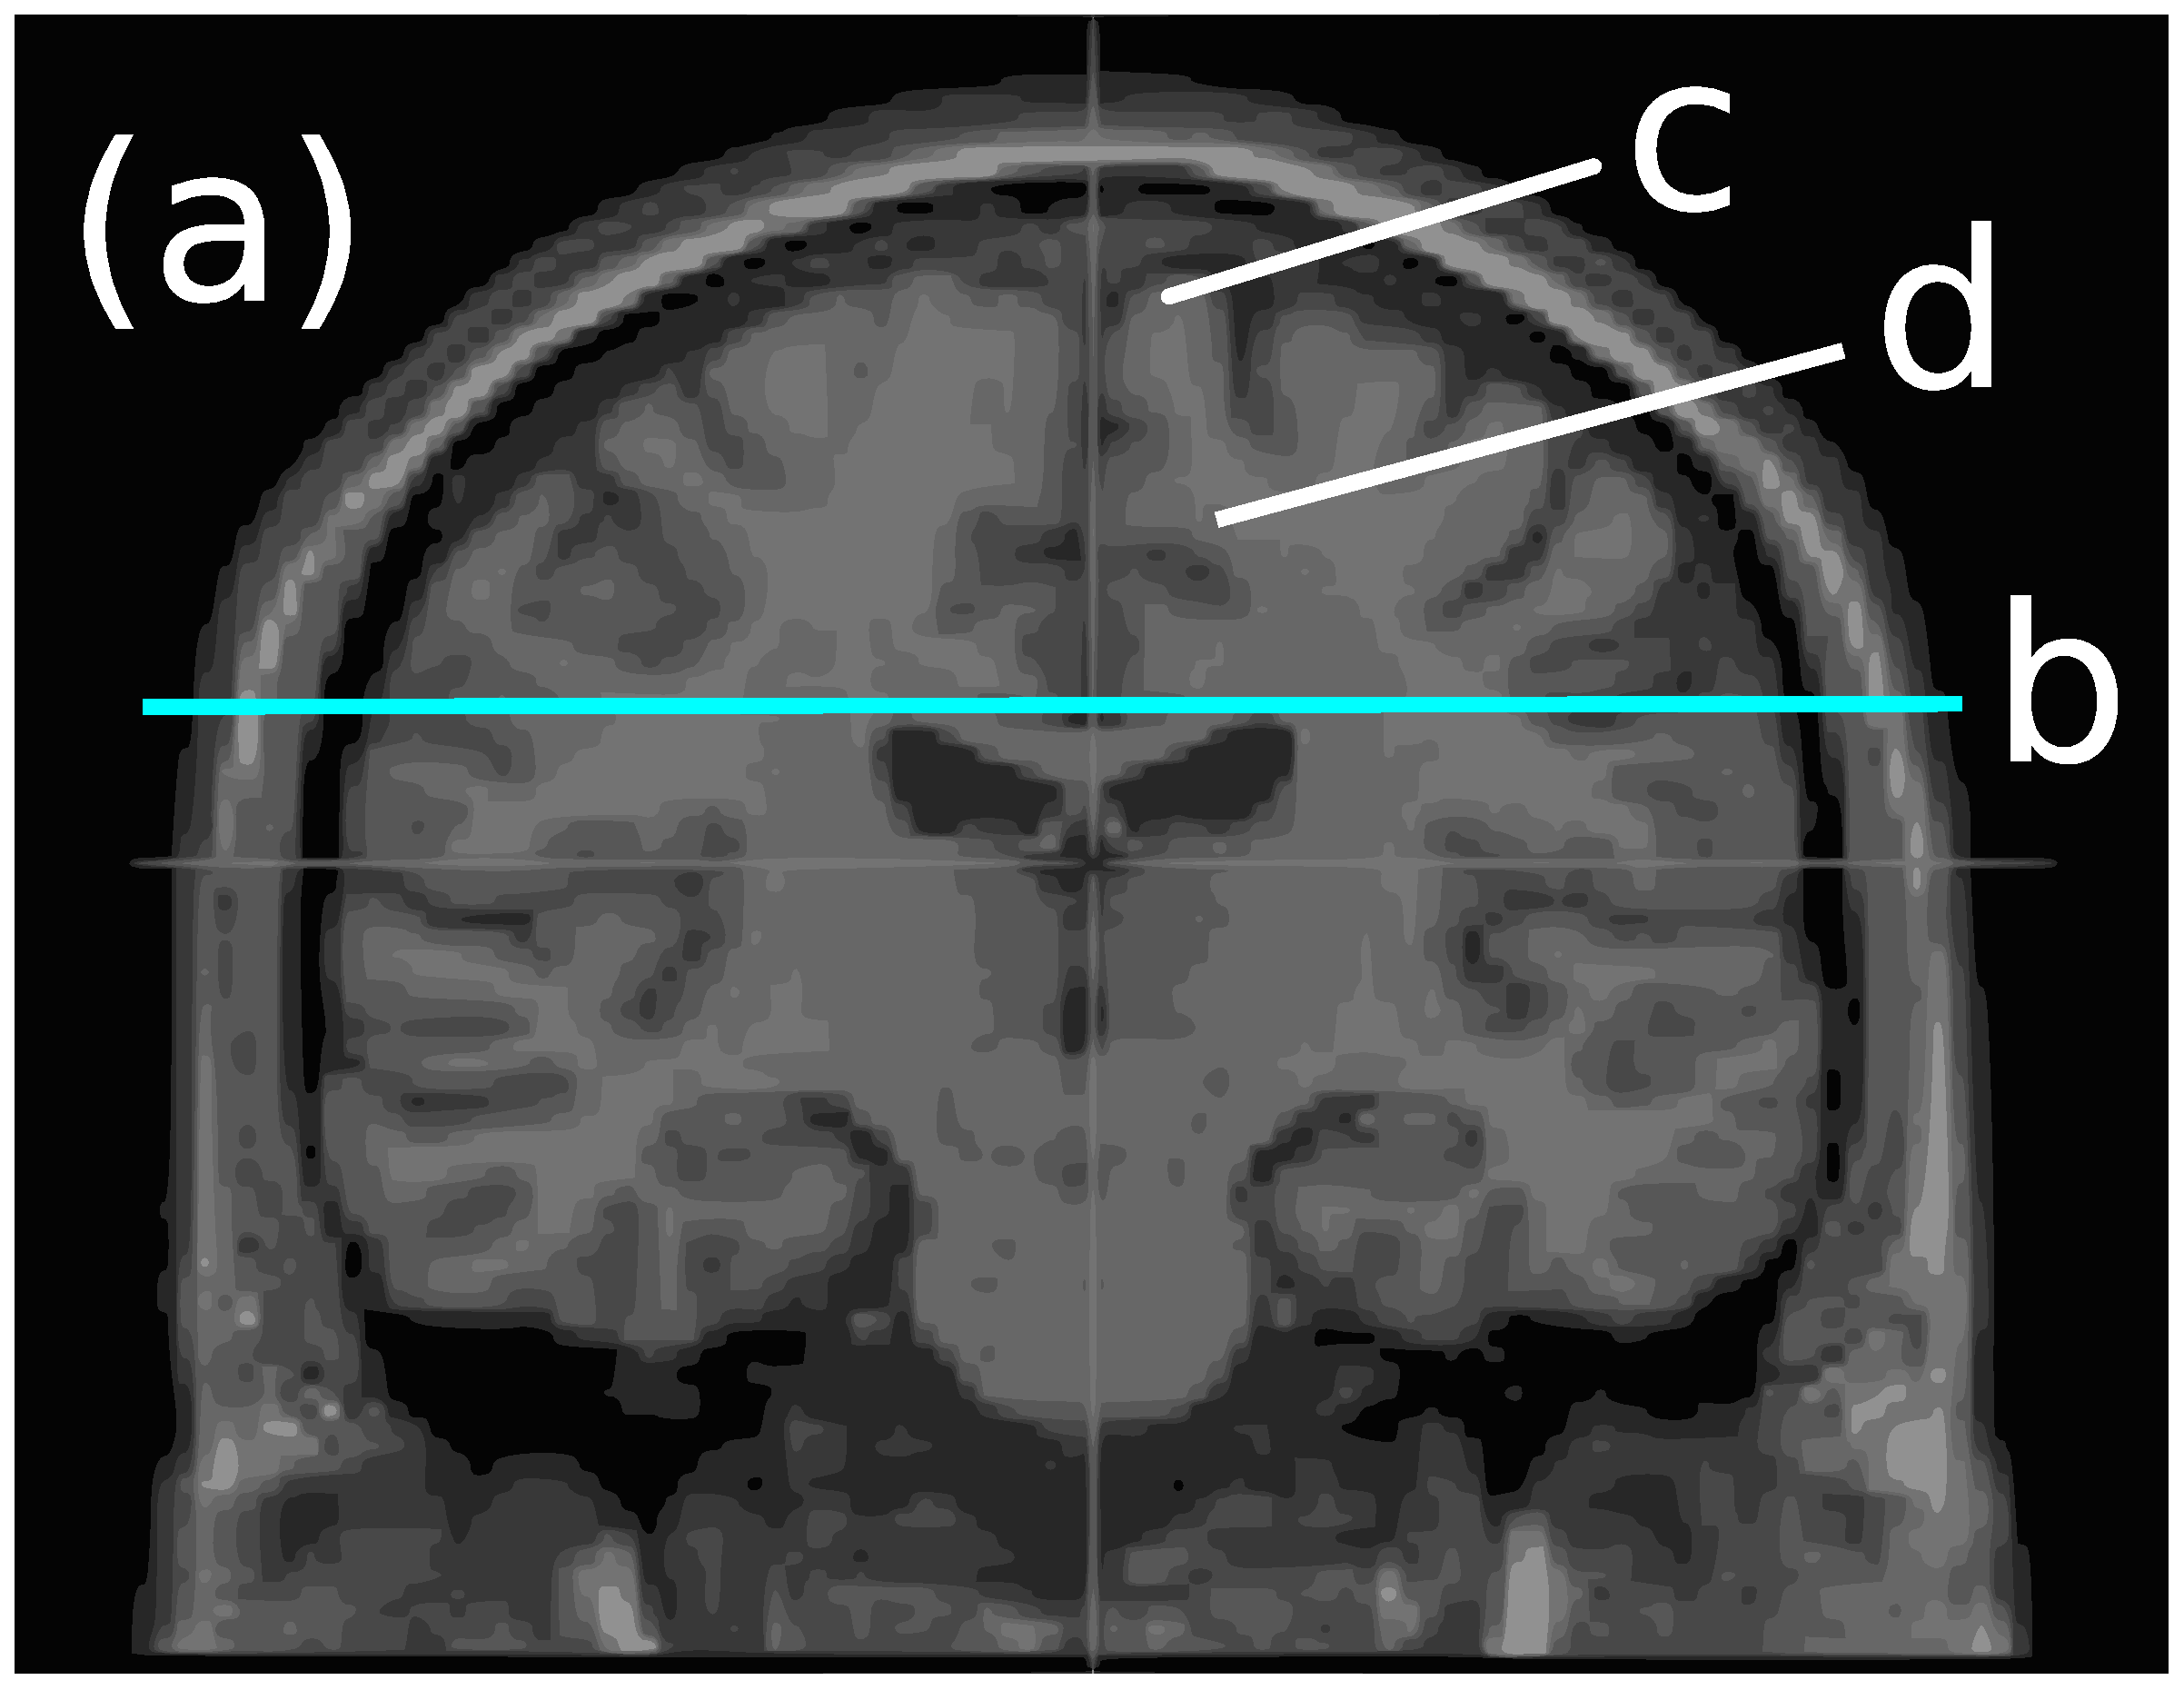
\includegraphics[width=0.36\textwidth]{headref}} & 
    			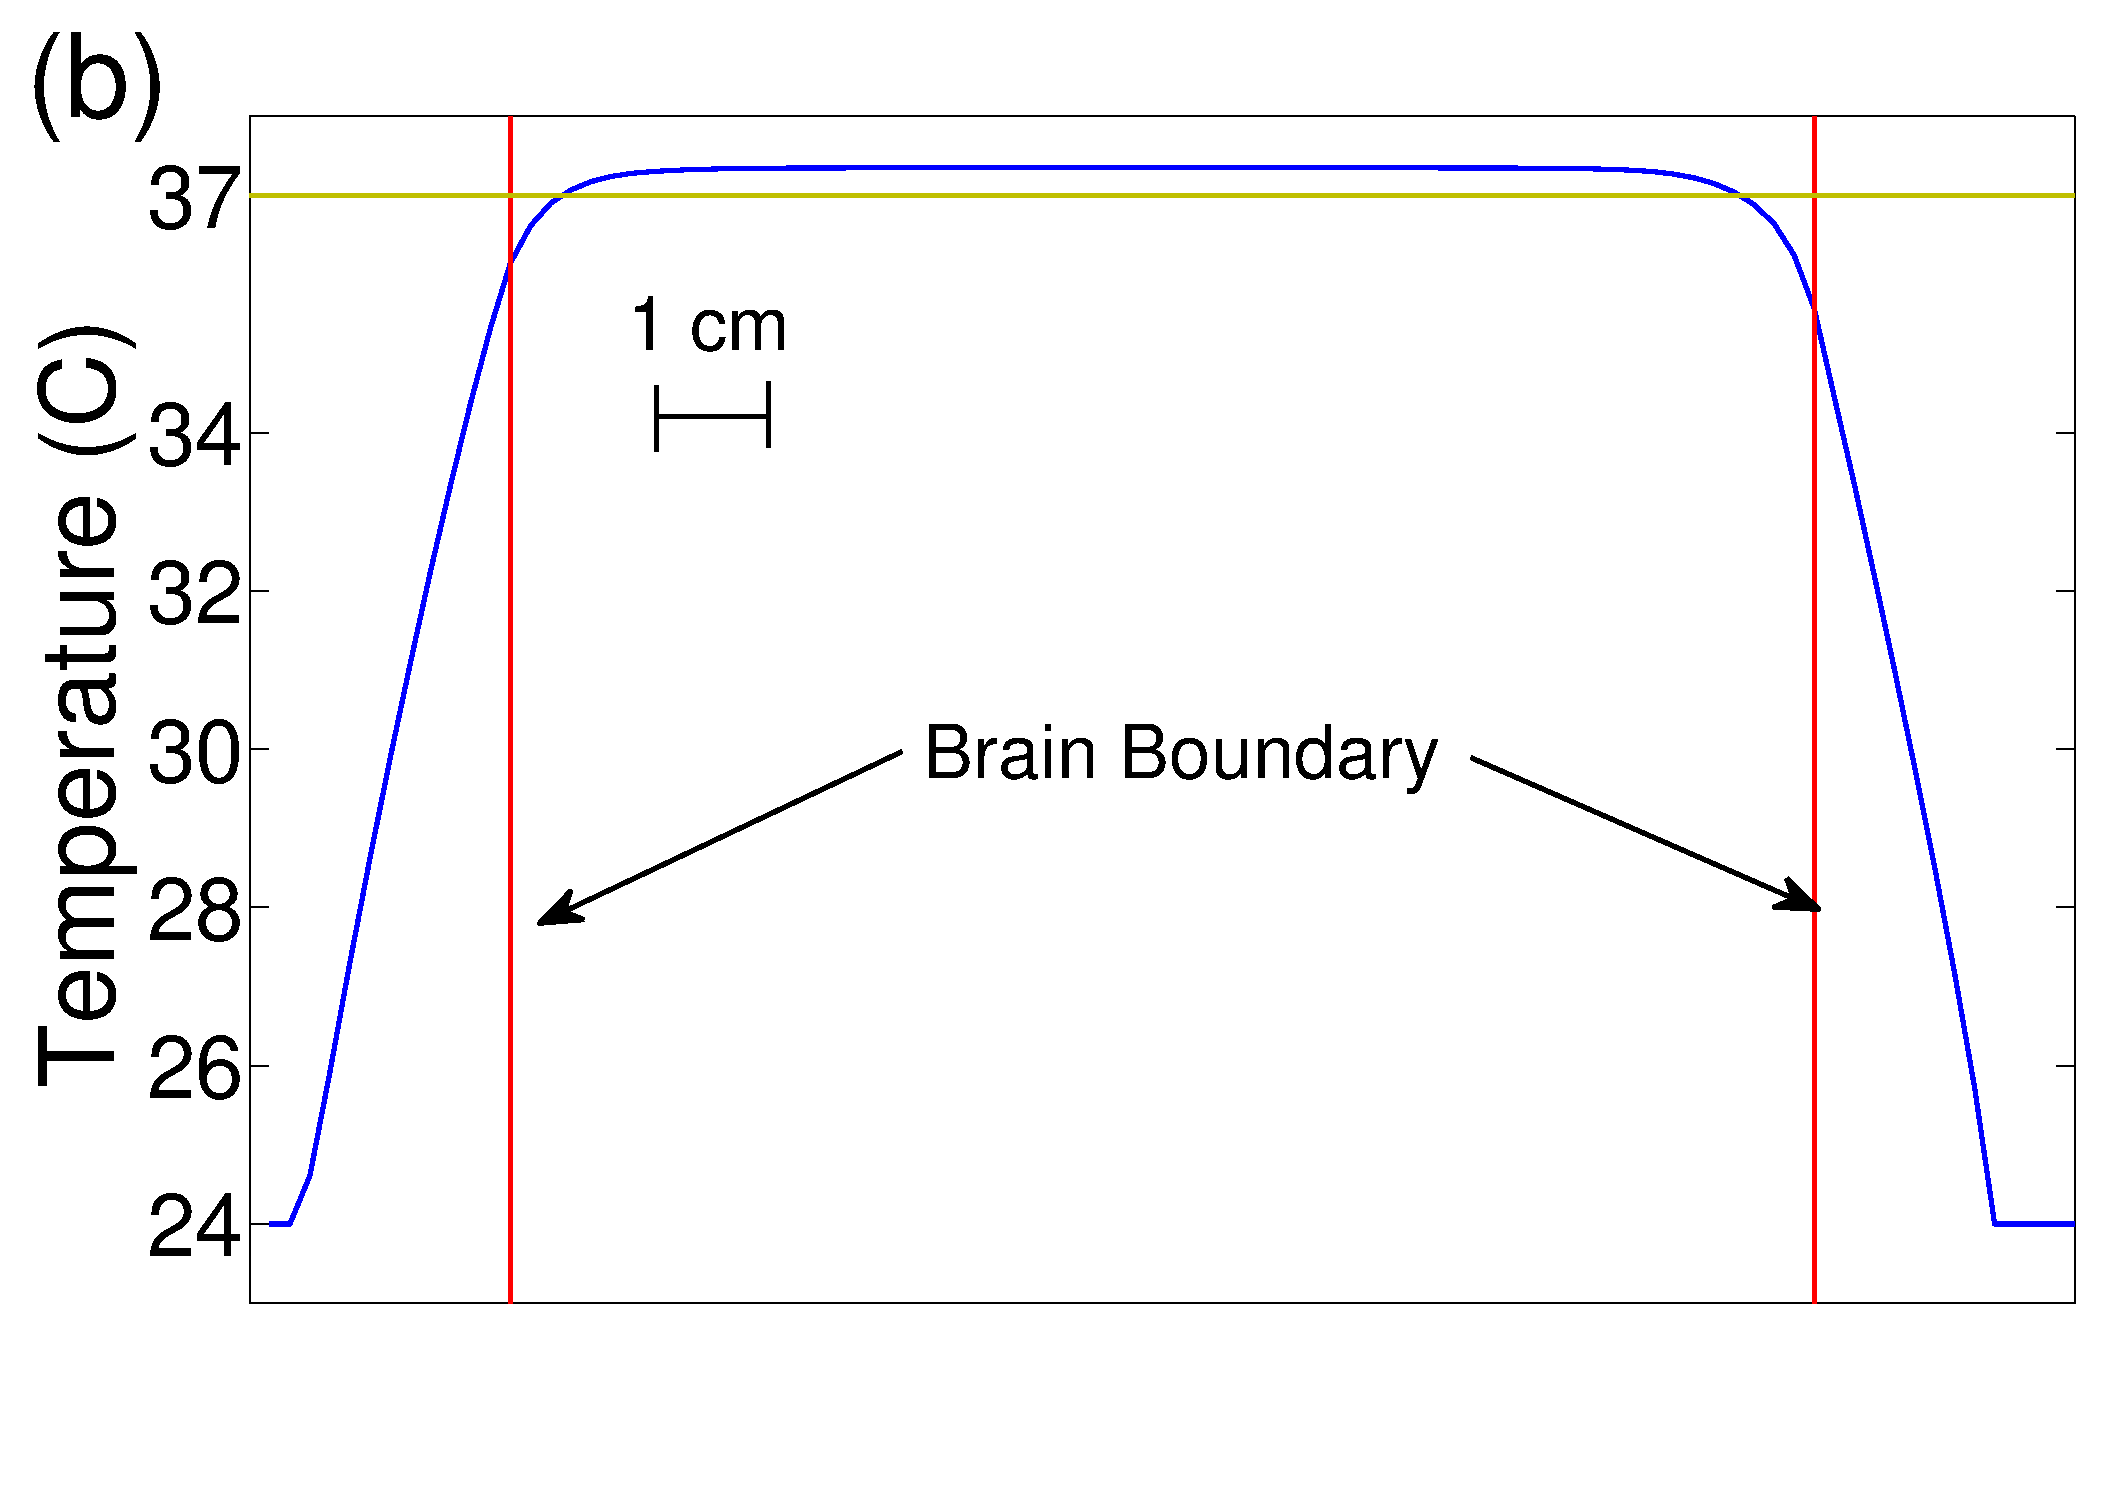
\includegraphics[width=0.5\textwidth]{equilibrium_temperature_0_55_52} \\
    			\multicolumn{2}{c}{\includegraphics{sim_bold_(48_58_76)}} \\
    			\multicolumn{2}{c}{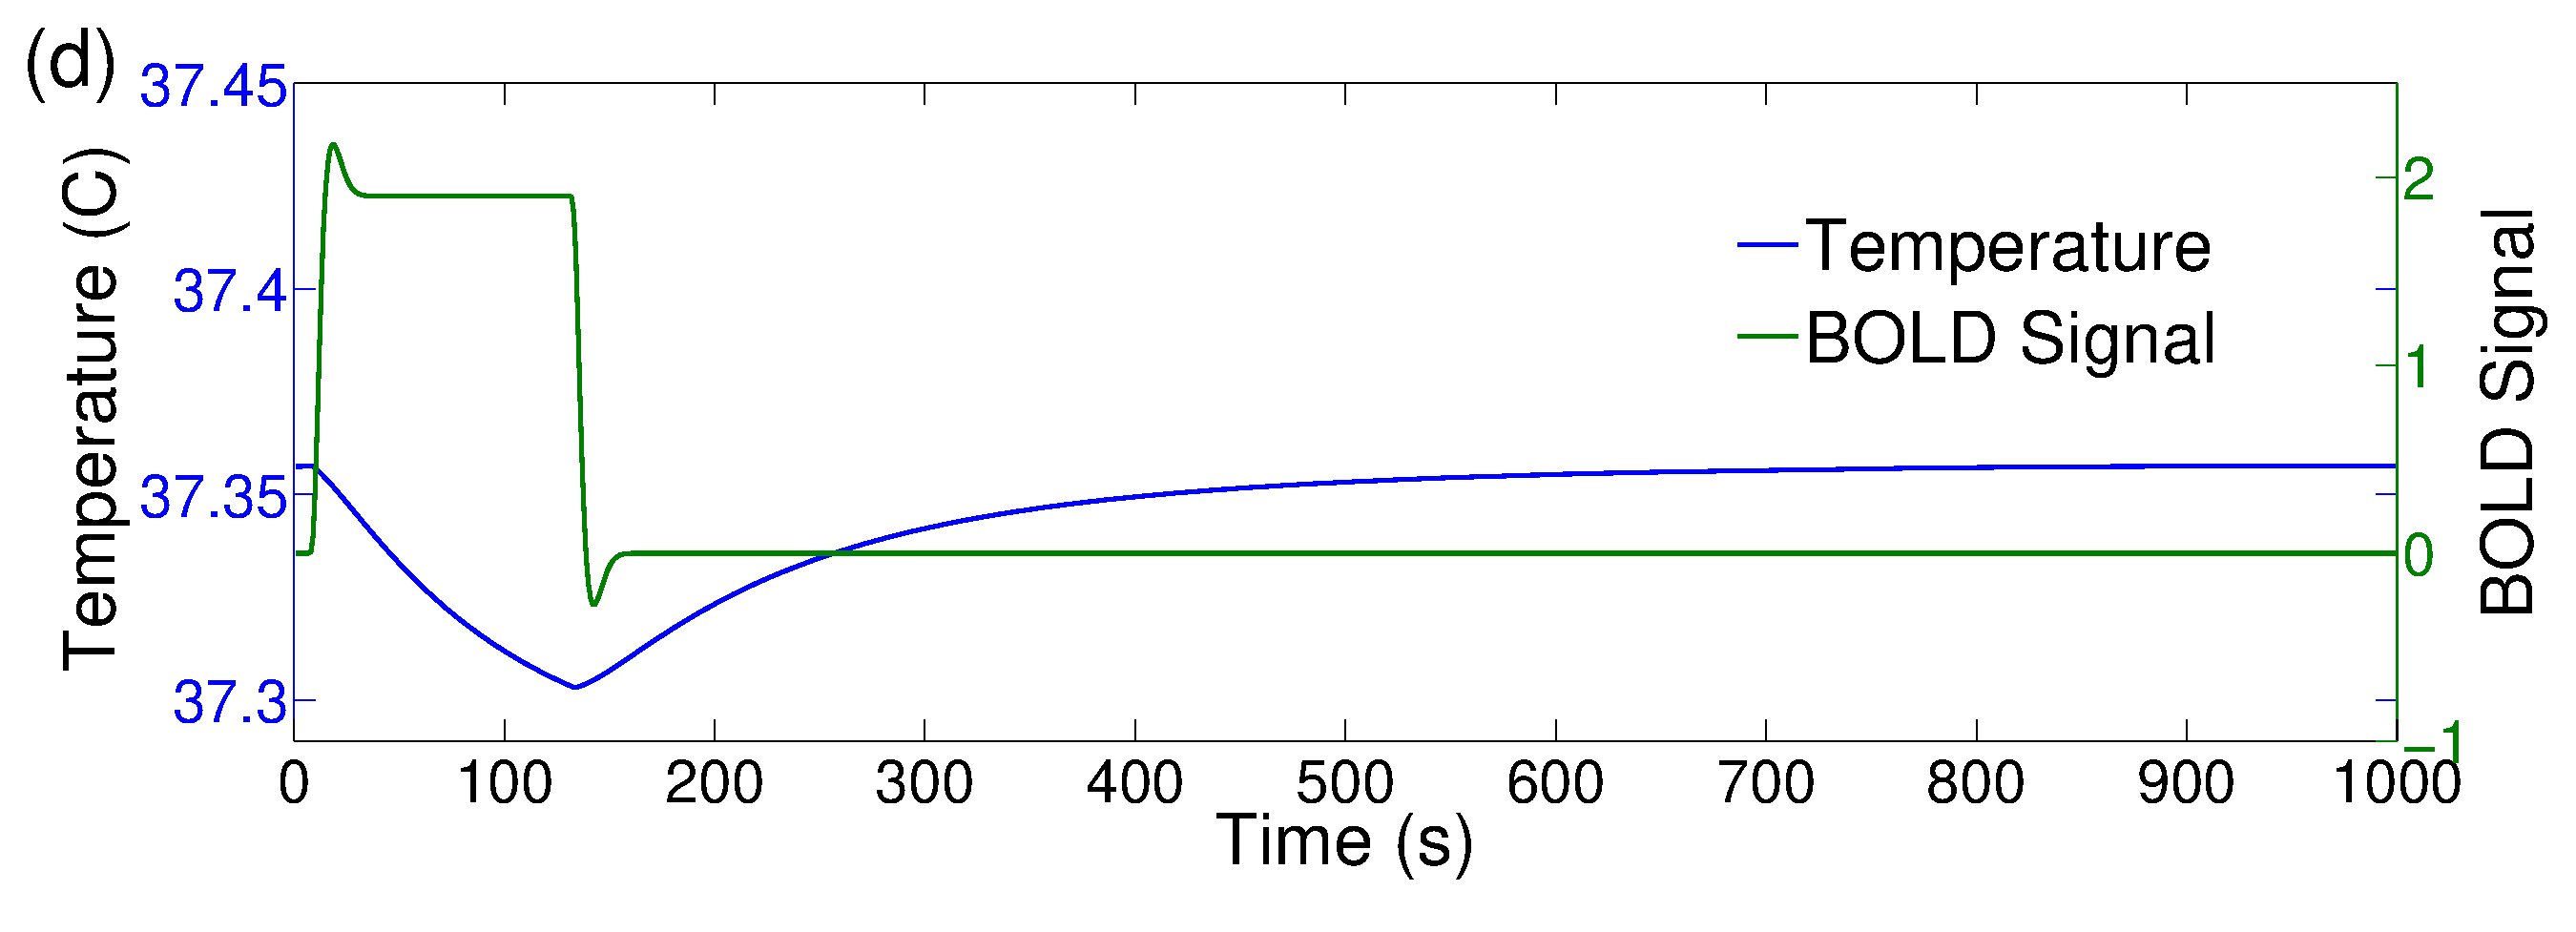
\includegraphics{sim_bold_(48_58_56)}}
    		\end{tabularx}
    	\end{center}
    	\caption[Temperature changes: simulated BOLD data]{\label{fig:simulateddata} Temperature changes using simulated BOLD signals. (a) Slice of the head (y = -12) with indicators of the locations for parts (b)-(d). (b) Equilibrium temperature along a line through the head. Red lines indicate the brain boundary and the gold line indicates the blood temperature (37\degree C) used for calculations. Inside the brain, a 4-6 mm thick shell is created where the equilibrium temperature is less than the blood temperature. Within this shell, (c) the temperature rises with increased brain activity while (d) tissue deeper in the brain experiences the opposite effect.} 
    \end{figure}
    To better understand the behavior of the tissue temperature model and the characteristics of temperature changes, BOLD activity was simulated in two ways: (i) from a nonlinear hemodynamic model \cite{friston2000} using stimulus or response function, or (ii) by convolving a boxcar function with the canonical hemodynamic response function provided by SPM 8 and corresponding temperature changes were calculated. Figure \ref{fig:simulateddata}(c,d) shows a typical simulated BOLD response used (green curve) along with the change in temperature (blue) for two voxels at different locations in the brain (locations indicated by Fig. \ref{fig:simulateddata}(a)). 
    
    Although both voxels have the same BOLD data, the demonstrate contrasting changes in temperature.  This can be best understood by considering the equilibrium temperature of each voxel.  Figure \ref{fig:simulateddata}(b) is a plot of the equilibrium temperature (blue line) along a line passing through the head (path indicated by the teal line in part (a) of the same figure). The vertical red lines indicate the boundary between the brain and surrounding tissues and the horizontal yellow line is an indication of the blood temperature (37\degree C). Two regions exist within the brain that lead to contrasting temperature behaviors.  
    
    The majority of the brain tissue is at a resting-state temperature that is less than the blood temperature (region 1).  For voxels within this region, a behavior like that shown in Fig.~\ref{fig:simulateddata}(d) is to be expected.  The primary contribution to an increase in the BOLD response is an increase in local blood flow.  Since the blood temperature is cooler than the tissue temperature, it removes heat from the tissue thereby lowering the temperature.  Single-voxel models are able to account for this result because their assumptions about the location of a voxel are consistent with being located within this region.
    
    The second region is comprised of a thin (4--6 mm) layer of brain tissue that is closest to the surface of the head.  As a result of its proximity to the surface of the head, conductive heat lost to the air puts the resting-state temperature of voxels in this region below the arterial blood temperature.  As a result, when there is an increase in blood flow (increase in BOLD), the warmer blood will increase the voxel temperature (Fig.~\ref{fig:simulateddata}(c)).  Since single-voxel models approximate voxel conditions, they are unable to account for this region of tissue.
    
    Conduction is a slow process, so over shorter time scales (less than ~10 minutes), conduction will contribute very little to the temperature change from a change in brain activity.  However, conduction plays an important role in determining the resting-state temperature.  
    
    The primary advantage with this model is that it accounts for the location of the voxel when determining the temperature, thus the direction of the temperature change depends on how far away from the surface of the head the voxel is. For voxels within a 4--6 mm shell near the surface of the brain, the temperature increases with increased activity (Fig. \ref{fig:simulateddata}(c)) while voxels deeper within the brain experience the opposite change (Fig. \ref{fig:simulateddata}(d)).
    
    %%  EXPERIMENTAl RESULTS %%
    \subsection{\label{sec:experimentalresults} Using Experimental BOLD Data}
    \FloatBarrier
    \begin{figure}[p] 
    	\begin{center}
    		$ 
    		\begin{array}{c}
    			\includegraphics[width=0.9\linewidth]{slice_x_24} \\
    			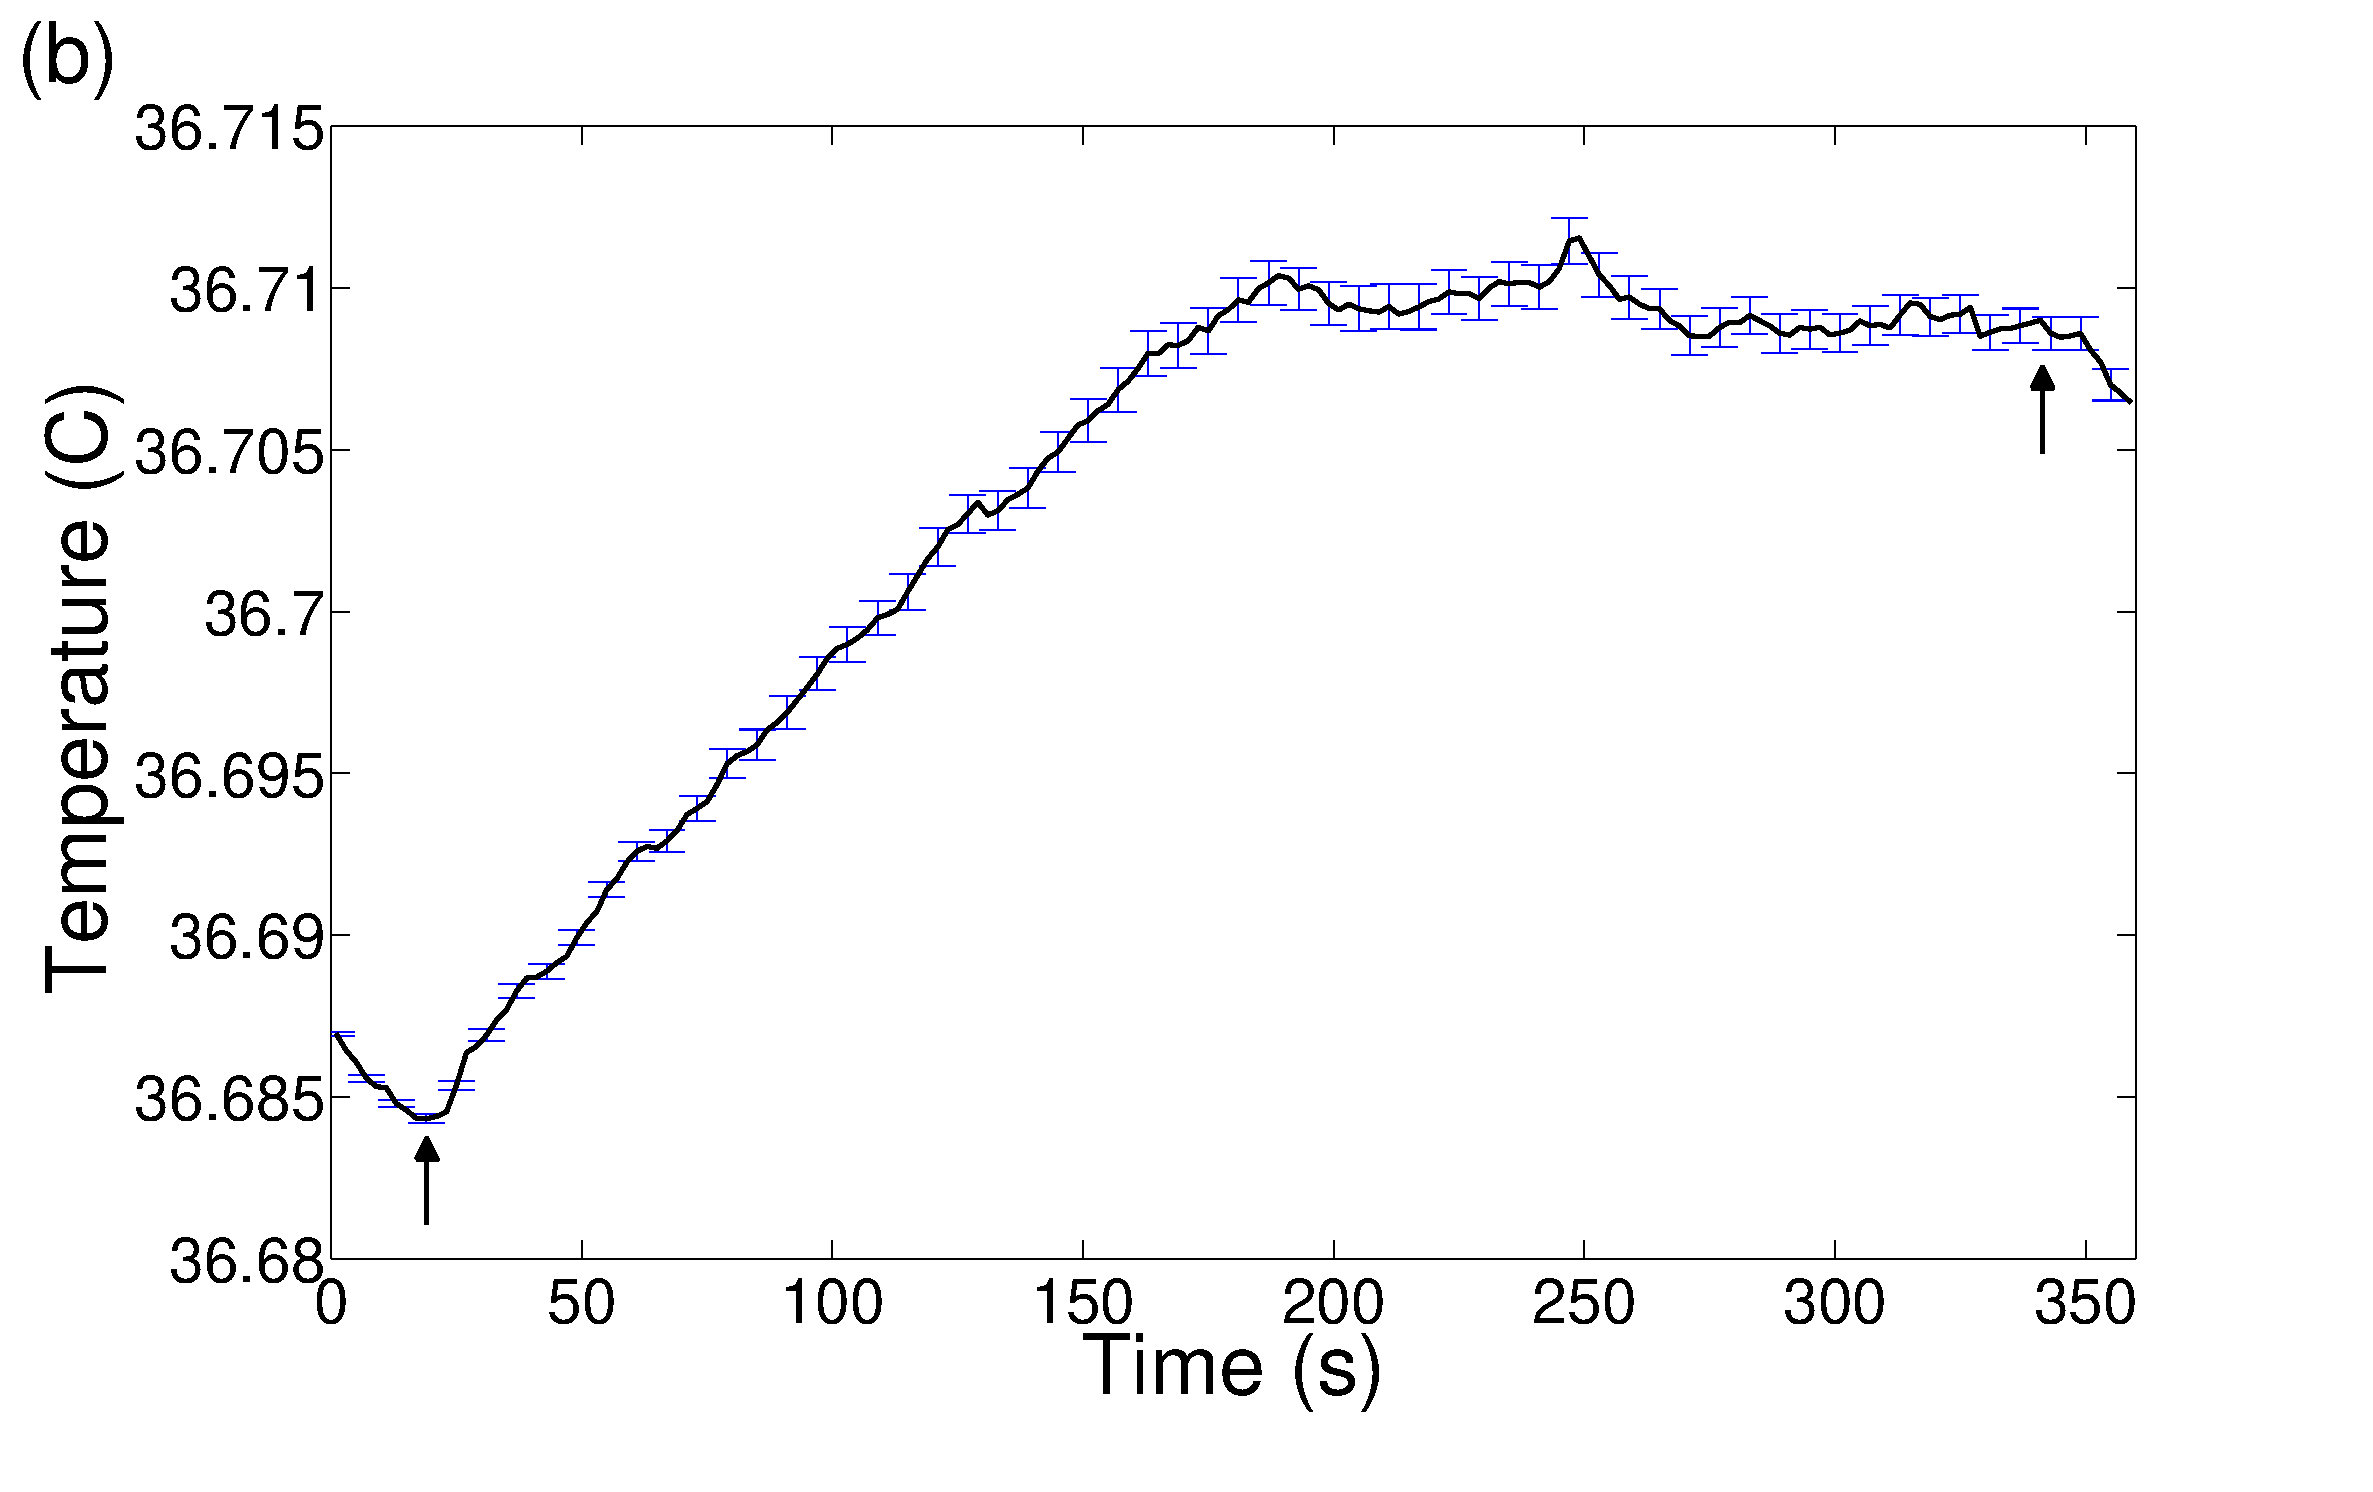
\includegraphics[width=0.9\linewidth]{avg_data_24_52_67} 
    		\end{array}
    		$ 
    	\end{center}
    	\caption[Temperature changes: experimental BOLD data]{\label{fig:realdata} Temperature calculated from a voxel within the motor cortex. (a) A slice (x = -44) showing the motor cortex warming during a finger-tapping task. (b) Temperature at a voxel within the motor cortex (-44, -24, 60) with standard error indicated by blue error bars (Arrows indicate task onset and conclusion, N=24).} 
    \end{figure}
    Data from a previous fMRI study~\citep{dhamala} was used to study the characteristics of temperature changes in a typical experiment. All participants in this experiment were right handed and between the ages of 23 and 27 years old.  Signed informed consent was collected from each one prior to participating in the study.  Institutional Review Boards of Emory University and Georgia State University approved this experiment. Twelve participants were asked to tap their right index fingers with rhythms of varying complexity for 320s. 
    
    This task resulted in a strong BOLD response in the motor cortex (\cref{fig:realdata}). The experiment included 20s of rest at the beginning and end of the tapping periods. Here, the resting state response level is calculated for each voxel by averaging across 40s of resting-state fMRI data. Using equations~\cref{eq:f,eq:m,eq:y}, the time-dependent change in blood flow and metabolism can be determined for each voxel. Finally, these values are used in conjunction with~\cref{eq:3dbioheat} to find the change in temperature throughout the brain. In this task, a temperature increase of approximately 0.02\degree C was observed in the motor cortex (\cref{fig:realdata}).  This value is well within the range of temperature changes observed in experimental measurements~\citep{mcelligott,kiyatkin,zeschke,george,tachibana}. 
    
    The increase rather than decrease in temperature in the motor cortex during a functional activity is consistent with the idea that the temperature of the blood in the capillaries is slightly greater than the baseline tissue temperature in superficial cortical regions; however, single-voxel models predict the opposite effect.
\clearpage\chapter{Optical Detector Applications to measuring the active brain}
\label{ch:detectors}
The most precise method for measuring brain temperature is to use a thermocouple probe placed in direct contact with the tissue.  The disadvantage of this method and the reason it  can not be used in humans is because it is invasive and damaging.  Thus, an optical method would be ideal since it is non-invasive and non-damaging.  Currently, there does not exist a method for accurately measuring the temperature of brain tissue optically.  However, other optical measurements methods could be used in conjunction with a temperature model (such as the one proposed here) to calculate the temperature.  The possible application of functional Near-Infrared Spectroscopy (fNIRS) and its possible use in brain temperature calculations is discussed along with the limitations of a direct measurement technique such as a thermal imaging camera.
  
\section{{F}unctional {N}ear-{I}nfrared {fNIR} Spectroscopy}
% detector applicaitons to improving fNIR
\begin{figure}[tb]
  \begin{center}
    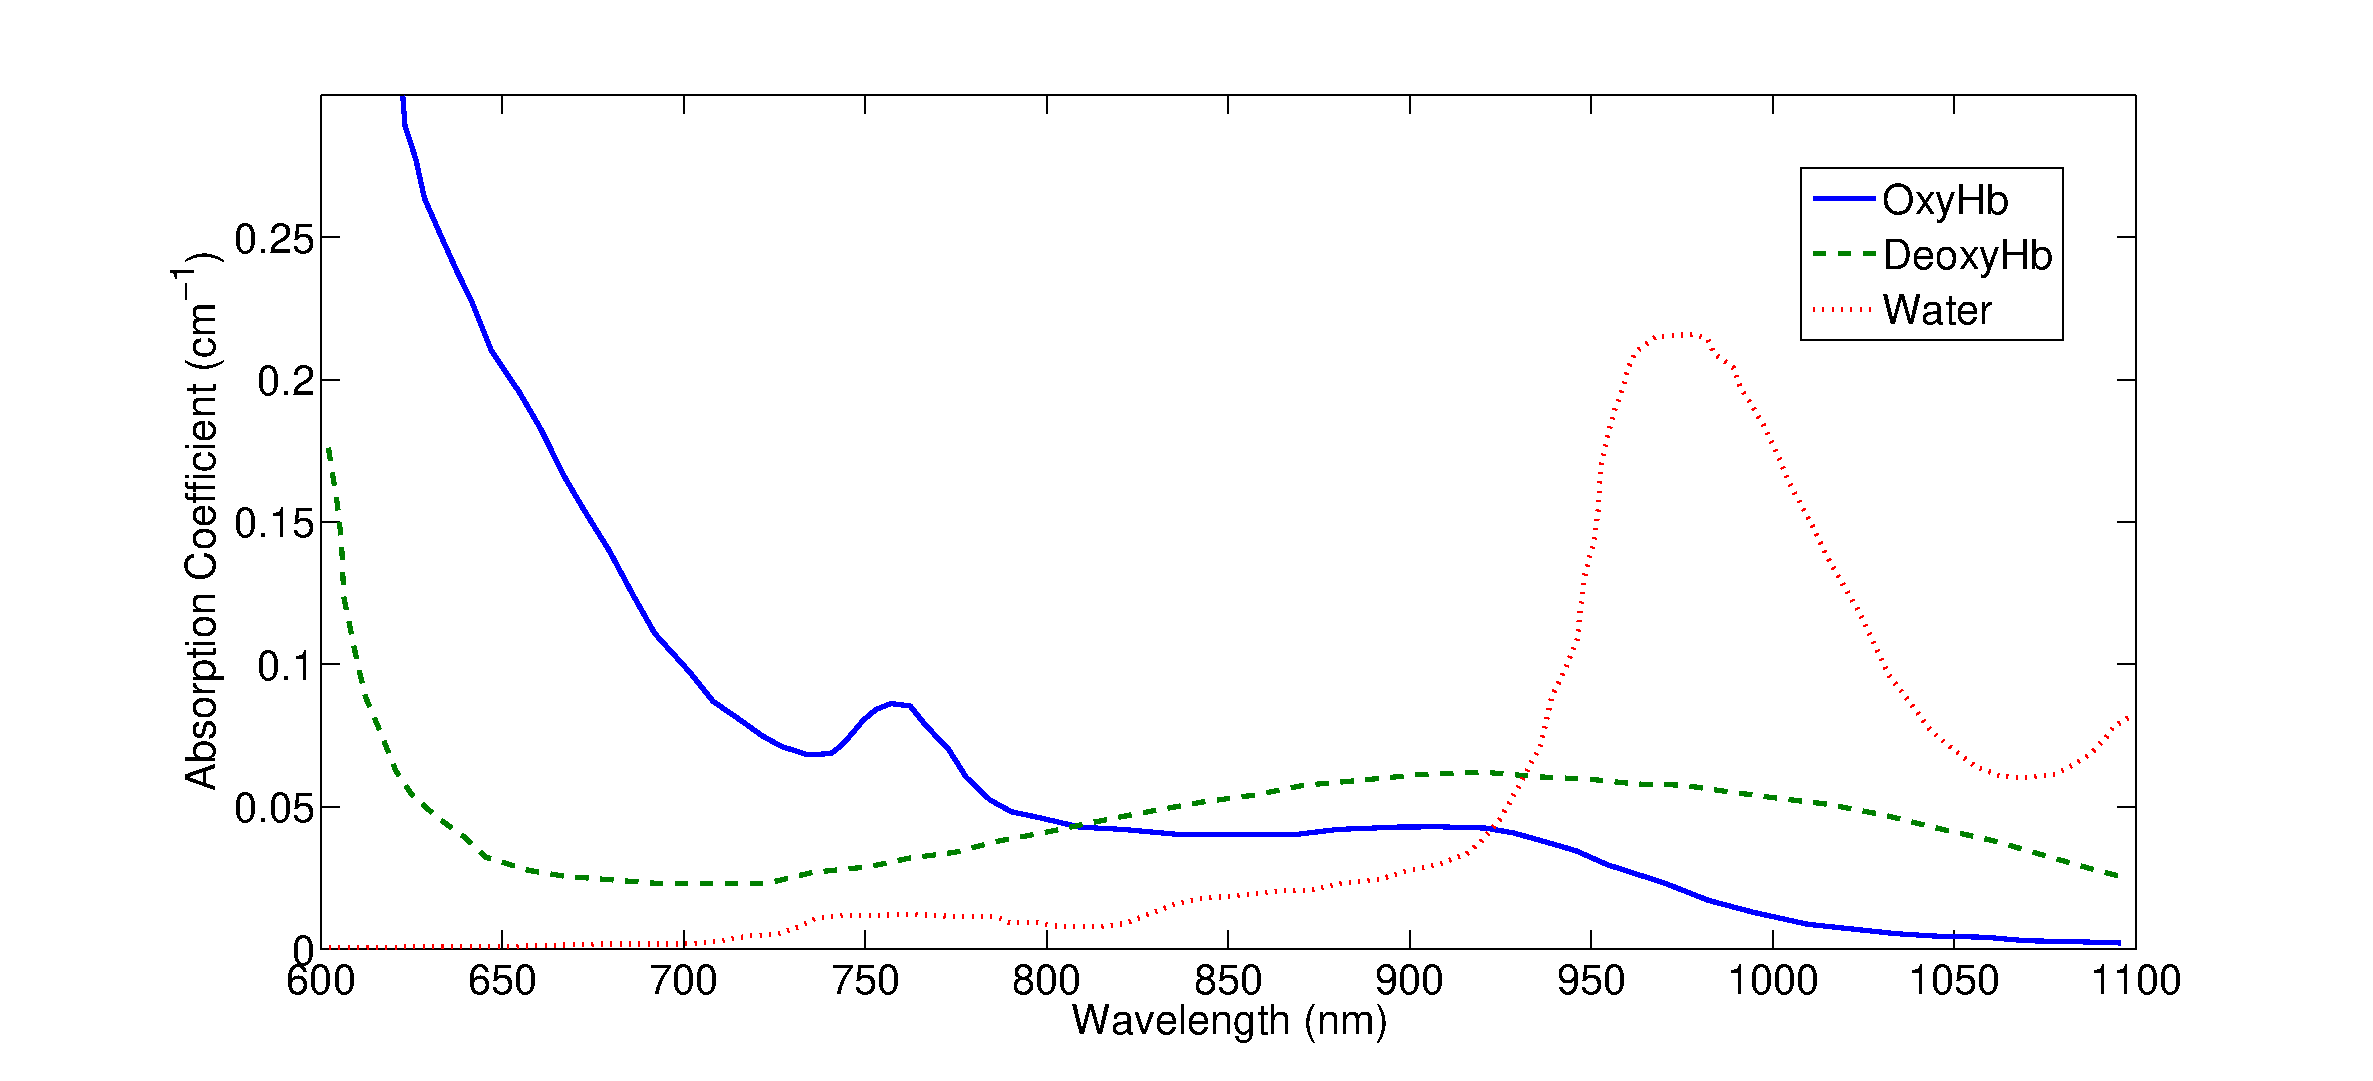
\includegraphics{AbsorptionData}
    \caption[Absorption spectra of water, deoxyhemoglobin and oxyhemoblogin]{\label{fig:fnirabsorption} Absorption spectra of water~\citet{cope}, oxyHb and deoxyHb~\citet{horecker}.}
  \end{center}
\end{figure}
\begin{table*}[tb]
  \begin{tabular*}{\linewidth}{lp{5cm}p{5cm}}
    \toprule
                         & fMRI             & fNIR            \\
    \midrule
    Spatial Resolution   & 8--27 mm$^3$  & $\sim$ 1--10 cm$^3$ \\
    Temporal Resolution  & 1--2 s        & $\sim$ 10$^{-3}$ s \\
    Measurement Parameter& blood volume, flow, and O$_2$ metabolism & oxyHb and deoxyHb concentrations \\
    Motion               & Must Remain Stationary & Small movements OK \\
    Penetration          & Whole-head    & outer 2--4 mm of brain tissue \\
    \bottomrule
  \end{tabular*}
  \caption[Comparison of fMRI and fNIR]{\label{tbl:comaparemethods}Comparison of the capabilities and limitations of fMRI and fNIR techniques.  Compiled from~\citet{bunce2006,elliott}.}
\end{table*}

As discussed in~\cref{ch:introduction}, changes in tissue activity can be detected by measuring the change in blood oxygenation levels.  Functional Magnetic Resonance Imaging (fMRI) is one technique for accomplishing this (the BOLD signal), but other techniques exist.  

Blood oxygenation can be determined by measuring the relative concentrations of oxyhemoglobin (oxyHb) and deoxyhemoglobin (deoxyHb).  Since oxyHb and deoxyHb have different absorption spectra (\cref{fig:fnirabsorption}), it is possible to determine this through optical techniques.  Functional Near-Infrared Spectroscopy is a technique which utilizes two or more spectral bands in order to determine blood oxygenation.  It has a high temporal resolution (millisecond), a low spatial resolution ($\sim$ 1~cm$^3$) compared to fMRI (as low as 1 mm$^3$), and is limited to only imaging the outer cortex (2--4 mm)~\citep{bunce2006}. A comparison of fMRI and fNIR is presented in~\cref{tbl:comaparemethods}.

fNIRS works by utilizing an array of near-infrared detectors and emitters (typically spaced 2--3 cm apart) placed in contact with the skin~\citep{villringer1997,izzetoglu2004}.  The exact spacing determines the depth the light is detected from.  As shown in~\cref{fig:fnirpenetration}, the closer the spacing, the higher the resolution but at the expense of lower penetration.  Conversely, in order to detect light passing through deeper tissue, a wider spacing is used which reduces the resolution.  The exact wavelengths used vary, but all lie within an optical window between 700--1000~nm~\citep{villringer1997} where absorption of near-infrared photons by tissue is low~(\cref{fig:fnirabsorption}).

\begin{figure}[tb]
  \centering
  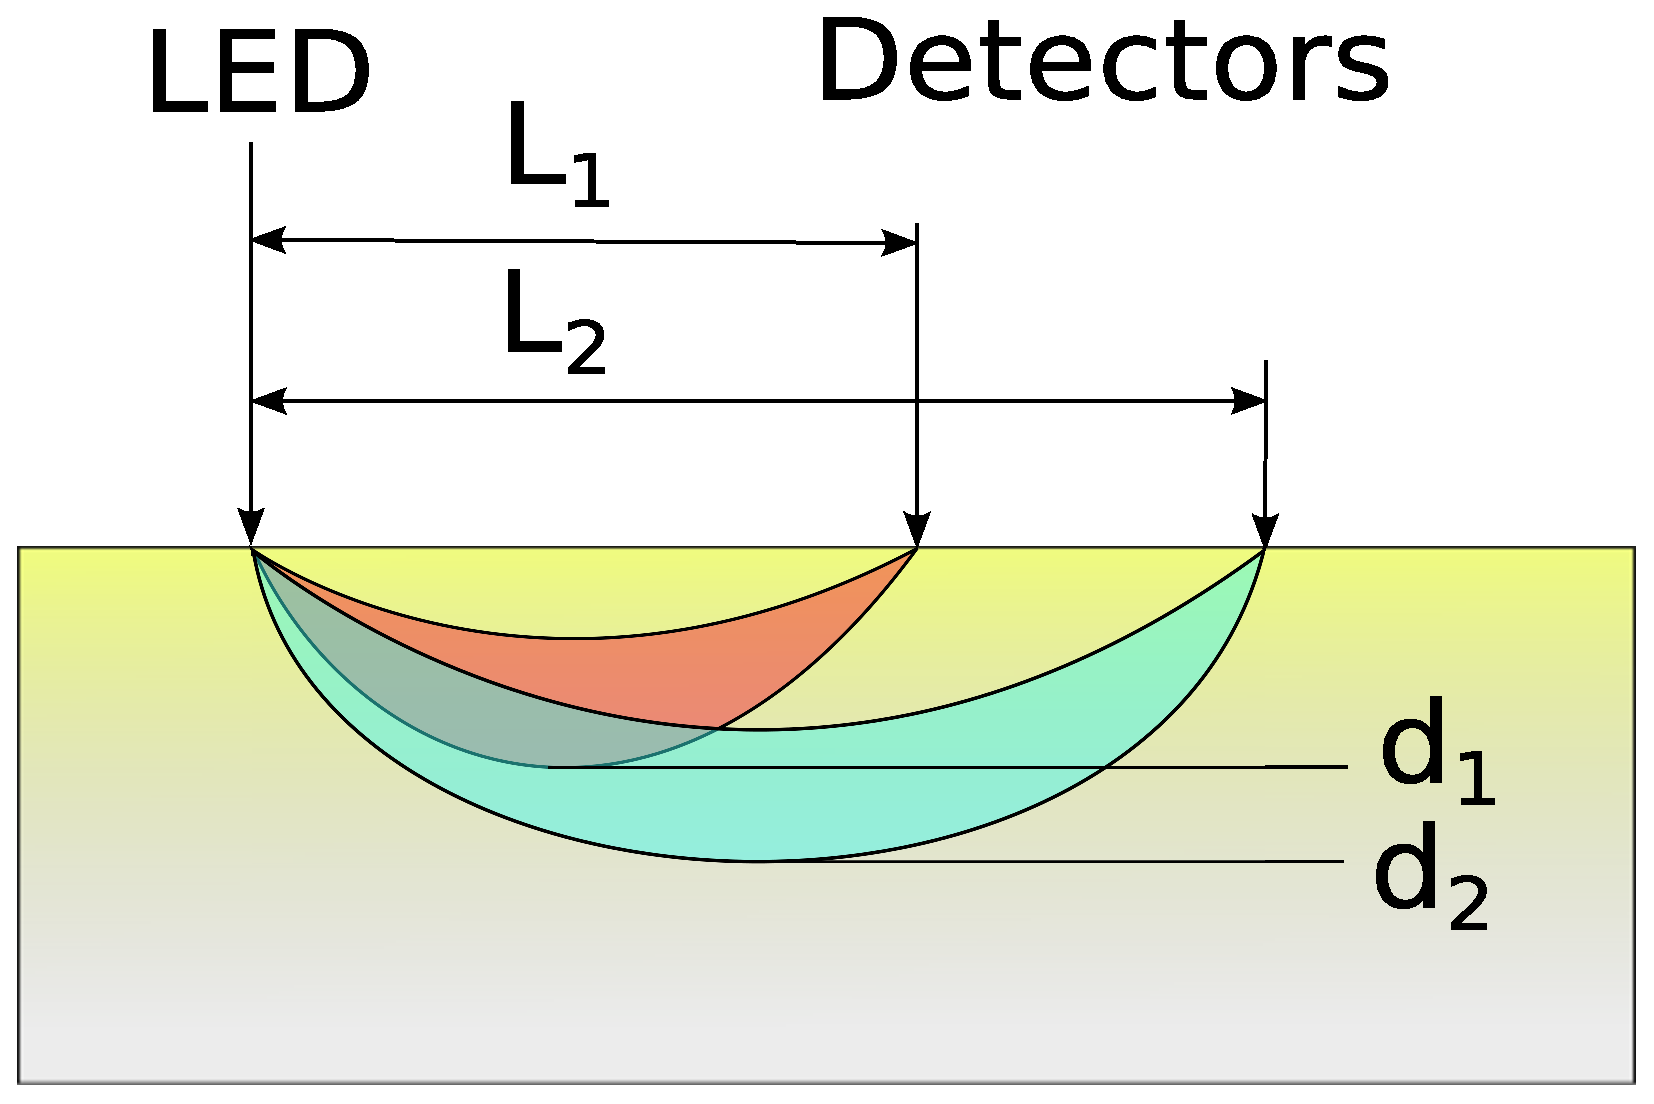
\includegraphics{fnir-penetration}
  \caption[Penetration by fNIR]{\label{fig:fnirpenetration}Penetration depth of a fNIR detector as a function of the distance between the NIR LED emitter and detector.  Modified after~\citep{head2010}}
\end{figure}

Three techniques are used to illuminate the tissue: (i)~time domain (or time resolved spectroscopy, TRS), (ii)~frequency domain and, (iii)~continuous wave illumination~\citep{izzetoglu2004}.  In TRS, short pulses of light are incident on the tissue and the temporal distribution of photons in measured.  In frequency domain spectroscopy, the amplitude of the indecent light is modulated at a high frequency (10--100~MHz) and the phase shift and amplitude decay of the detected light is compared to the incident light~\citep{boas2002}. In continuous wave illumination, the incident light is not modulated so the detected light can only be compared for amplitude attenuation~\citep{izzetoglu2004}.

All of the techniques use a modified version of the Beer-Lambert Law~(\cref{eq:beerlambert})~\citep{cope}.  
\begin{equation}
  \label{eq:modifiedbeerlamber}
  I = G I_0 e^{-(\alpha_{deoxyHb}C_{deoxyHb}+\alpha_{oxyHb}C_{oxyHb})L} 
\end{equation}
where G is a factor to adjust for the measurement geometry, $I_0$ is in the incident light intensity, $\alpha_{oxyHb}$ and $\alpha_{deoxyHb}$ are the molar extinction coefficients for oxyHb and deoxyHb, $C_{oxyHb}$ and $C_{deoxyHb}$ are the chromophore concentrations for oxy-Hb and deoxy-Hb, and L is the path length~\citep{izzetoglu2004}.  By comparing a baseline measurement~($I_b$) with a new measurement~($I$), the optical density can be determined~\citep{izzetoglu2004}
\begin{equation}
  \Delta OD = \log \frac{I_b}{I} = \alpha_{deoxyHb} \Delta C_{deoxyHb}+\alpha_{oxyHb} \Delta C_{oxyHb}
\end{equation}
As discussed in~\citet{izzetoglu2004}, at least two wavelengths are utilized in the spectral window (700--1000~nm) in order to determine the change in concentration of chromophores $\Delta C_{deoxyHb}$ and $\Delta C_{oxyHb}$.  With these values, the oxygenation and total blood volume can be determined:
\begin{align}
  \label{eq:o2bloodvolume}
  Oxygenation\ &= \Delta C_{HBO2} - \Delta C_{HB} \nonumber \\
  Blood\ Volume\ &= \Delta C_{HBO2} + \Delta C_{HB} 
\end{align}
Using this method to experimentally measure the blood oxygenation while measuring the fMRI BOLD response could be used to better refine the current model for calculating the metabolism and blood flow from the BOLD response.

While fNIRS does not provide as spatially-precise a measurement as fMRI, it should be possible to modify the existing model for calculating temperature from the BOLD response to use fNIR data. This would be advantageous because fNIRS systems are cheaper and less disruptive than fMRI systems, meaning they can be used with a wider range of patients (children and the elderly).  For this reason, developing a model which uses fNIRS data should be considered in future research.

\section{Thermal Imaging}

The primary challenge in brain temperature research is making experimental measurements of brain temperature.  The most accurate modality is to use a thermocouple probe, but since this is invasive and causes tissue damage, it is not possible to use this technique with human subjects.  For this reason, a non-invasive technique such as a thermal imaging camera is appealing.  Unfortunately, this technique is limited by the high absorption of mid-infrared photons by water.

Light absorption by a material is modeled using the Beer-Lambert law
\begin{equation}
  I = I_0 e^{-\alpha (\lambda) x} \label{eq:beerlambert}
\end{equation}
where $I$ is the intensity at a depth $x$ remaining from light with an incident intensity $I_0$ in a material with absorption coefficient $\alpha$.  The point at which the intensity has decayed to 1/$e$ (about 37\%) of the incident intensity is called the penetration depth, $\delta_{p}$
\begin{equation}
  \delta_p = \frac{1}{\alpha (\lambda)} \label{eq:penetrationdepth}
\end{equation}
This equation can be used along with the black body spectrum at tissue temperatures (\cref{fig:blackbody}) we can estimate the penetration depth of mid-infrared photons passing through water.

\begin{figure}[tb]
  \centering
  \includegraphics{blackbody310K}
  \caption[Black-body Spectrum at 310 K]{\label{fig:blackbody}Black-body spectrum at 310 K calculated using Planck's Law.}
\end{figure}
\begin{figure}[tb]
  \centering
  \includegraphics{water-wide-band}
  \caption[Wide-band absorption spectra of water]{\label{fig:waterabs}The absorptions spectra of water from UV to far-infrared.  Modified from~\citet{hale73}.}
\end{figure}

Wien's Displacement Law is a solution to Planck's law for the peak light emission wavelength:
\begin{align}
  \lambda_{max} &= \frac{b}{T} \label{eq:wienslaw} \\
  b &= 2.897\,7721 * 10^{-3} \mbox{ K m} \nonumber
\end{align}
where $b$ is Wien's displacement constant and T is the temperature in kelvin.  For $T=310$~K ($T=37\degree$~C), Wien's law yields a peak black-body emission wavelength of 9.35~\textmu m.  

Using~\cref{fig:waterabs} to find the absorption coefficient of approximately 700~cm$^{-1}$.  With the absorption coefficient, the penetration depth (\cref{eq:penetrationdepth}) is approximately 0.14~\textmu m.  This depth is roughly five orders of magnitude smaller than the distance from the surface of the brain to the surface of the head.  Thus, it can be assumed that a thermal imaging camera is unable to image photons coming from the brain.

When a thermal imaging camera is used, the photons collected come from the skin of the head rather than from any deeper tissues, thus it is not a viable form of brain activity detection unless direct line of sight to the brain is available (such as in an open skull surgery).  In this case, the temperature sensitivity of currently available cameras is greater than 14~mK~\citep{flir,ici} so it would be limited to only the most extreme of excitations.  As a comparison, the finger-tapping task discussed in the results section (\cref{sec:experimentalresults}) only induced a peak temperature change of 25~mK after tapping for about 170~seconds.  Detection of this activity would be at the limits of a thermal imaging camera.

While its applications to detecting brain activity are limited, thermal cameras could find use in the operating room.  It has been found that inducing mild hypothermia in patients being treated for cerebral ischemia improves the clinical outcome~\citep{maher1993}. The same treatment has been shown to improve the outcome of patients who have experienced a stroke~\citep{krieger2001}. Currently, the temperature of the brain is inferred from the core body temperature (which is monitored via an invasive thermistor catheter). If it is possible to directly image the brain (i.e. during surgery) then the hypothermia treatment can be better monitored through a thermal imaging camera.  This would be especially useful since conductive and radiative heat loss to the air from an exposed brain could reduce how tightly regulated the brain temperature is by the arterial blood temperature.

Optical detectors face many challenges working with biological tissue, the worst being infrared light absorption by water. fNIRS works within an optical window in the water absorption in order to measure changes in blood oxygenation, while thermal imaging is limited to measuring the temperature of tissue it has direct line of sight with because of the high absorption of water in the operating window. Despite their limitations, both of these techniques could be used in future studies to improve our understanding of brain temperature dynamics.
\clearpage\chapter{Conclusion}
Lorem ipsum dolor sit amet, consectetur adipiscing elit. Nulla ligula lorem, malesuada non feugiat a, bibendum sit amet leo. Sed in dui lacus. Nullam quam dolor, elementum ac semper vitae, lacinia et dui. Curabitur accumsan urna nec dolor porttitor mollis. Nunc id feugiat tellus. Proin orci arcu, egestas a tincidunt eu, luctus ut ligula. Curabitur at risus non nulla congue facilisis sed eu velit. Morbi eget bibendum sem.

Cras vel lectus leo. Donec at ante vel eros condimentum dignissim et at libero. Nullam vitae purus at diam semper gravida. Ut venenatis dapibus nulla pretium eleifend. Nam scelerisque dignissim augue, ac suscipit tellus vestibulum vel. Sed rutrum sollicitudin sodales. Pellentesque cursus lobortis neque, id ornare purus laoreet eget. Sed adipiscing sollicitudin convallis. Quisque eu orci sit amet libero mollis tincidunt. Nullam sed consectetur odio. Etiam a molestie orci.

Pellentesque sed purus odio. Nam pharetra aliquam augue vitae porta. Phasellus malesuada rhoncus tristique. Donec cursus, nibh vel eleifend bibendum, ante massa imperdiet mauris, vel varius dolor libero feugiat nibh. Sed libero sem, bibendum eu cursus sit amet, euismod in dui. Vestibulum massa nisl, accumsan eu cursus nec, pretium blandit lectus. Phasellus vitae ipsum eget tellus consequat molestie vel nec tortor. Curabitur blandit, lectus lacinia consectetur varius, leo metus placerat nisl, ullamcorper egestas nisl nisi in nulla.

Nunc sit amet mi sed ante dictum luctus eget et augue. Morbi vitae nunc justo. Praesent ac elit lorem. In hac habitasse platea dictumst. Integer pellentesque eros viverra justo scelerisque mollis. Vestibulum tempor tempus velit, et pulvinar odio iaculis ut. Quisque luctus massa sit amet justo ornare nec posuere eros aliquam. Vestibulum luctus pharetra augue, et varius ligula sollicitudin sit amet. Cras mi enim, laoreet quis vulputate ut, pulvinar vel nibh.

Cras sem justo, ultricies eget sodales eget, bibendum non neque. Pellentesque tempus mi eget massa venenatis id cursus sem aliquet. Nunc venenatis, est at porta faucibus, erat sem ultrices magna, eget tincidunt orci lorem vitae nisl. Sed sem velit, fermentum in hendrerit eu, tempor fermentum arcu. Nullam id nunc vel purus aliquet faucibus. Donec ullamcorper odio ac purus tristique mollis. Class aptent taciti sociosqu ad litora torquent per conubia nostra, per inceptos himenaeos. Pellentesque eget elit in orci iaculis congue. Suspendisse sit amet nisl a velit tempus pretium. Suspendisse quis vulputate nunc. Phasellus quis elit sit amet arcu faucibus adipiscing. Vestibulum faucibus enim ut libero venenatis ac facilisis dolor ultrices.
% Bibliography
\bibliographystyle{unsrtnat}
\clearpage\phantomsection
\addcontentsline{toc}{chapter}{References}
\bibliography{thesis}
\appendix
\clearpage\appendix
\addappheadtotoc
\chapter{Code}
\label{appendix:code}
The following sections include the code used.  It was written for Matlab R2011b and requires SPM8 to run.  Additionally, it is recommended that you have at least 4 GB of RAM in order to work with the large datasets that are produced.  For information about how to visualize the data produced, see~\cref{ch:visualize}.  All of the code is available through the temptools github page (\url{https://github.com/greggroth/temptools}).  Additionally, many of the tasks can be completed using the temptools gui (\cref{fig:ttmain,fig:ttcalcequil,fig:tttempcalc,fig:ttvisualize}) which can be invoked by running
\begin{lstlisting}[style=snippet]
  temptools
\end{lstlisting}
at the Matlab command prompt (make sure the temptools directory and subdirectories have been added to the Matlab path).  The procedure used is explained in~\cref{sec:approach} and a graphical representation is available in~\cref{fig:procedureflowchart}.
\begin{figure}[hbt]
  \centering
    \caption[temptools: main window]{\label{fig:ttmain} The main window of temptools.  From here, you can go through the calculation steps and launch the visualization tool.}
    \includegraphics[keepaspectratio=true, width=17cm]{temptools/main.png}
  \centering
\end{figure}
\begin{figure}[hbt]
  \centering
    \caption[temptools: calculate the equilibrium temperature window]{\label{fig:ttcalcequil} This is the interface for calculating the equilibrium temperature (method explained in~\cref{sec:findequil}) under certain conditions.}
    \includegraphics[keepaspectratio=true, width=17cm]{temptools/calcequil}
  \centering
\end{figure}
\begin{figure}[hbt]
  \centering
    \caption[temptools: calculate temperature during activity]{\label{fig:tttempcalc} The interface for calculating temperature changes when blood flow and metabolism are time dependent.  This can be achieved by either loading metabolism and blood flow datasets or by using generated activity.}
    \includegraphics[keepaspectratio=true, width=17cm]{temptools/tempcalc}
  \centering
\end{figure}
\begin{figure}[hbt]
  \centering
    \caption[temptools: visualize the data]{\label{fig:ttvisualize} Visualize your data using the temptools visualization window.  This loads all of the required data and launches a slice browser or tsliceplot (see \cref{ch:visualize} for more details).}
    \includegraphics[keepaspectratio=true, width=10cm]{temptools/visualize}
  \centering
\end{figure}
% Load T1/create head data
\section{Creating the Head Matrix}
\label{sec:headmatrix}
Before any calculations can be done, a matrix containing tissue-specific parameters must be created.  First, a T1 contrast image should be segmented using SPM8 (\url{http://www.fil.ion.ucl.ac.uk/spm/software/spm8/}).  For ease of consistency, the one provided by SPM8 in ./canonical/ is best to use.  Using SPM's ``New Segmentation'' algorithim will segment the image into five different tissue types (gray matter, white matter, cerebral spinal fluid, soft tissue and bone).  Once this is complete, run ImportSegmentedT1() within this directory and it will return a matrix that has been populated with the tissue-specific parameters required for accurate temperature calculations. The functions fillAir() (\ref{ass:fillair}), fillHoles() (\ref{ass:fillHoles}), build\_skin() (\ref{ass:buildskin}) and repair\_headdata() (\ref{ass:repairheaddata}) are functions required by BulkImportNII().  More information about this procedure is in~\cref{sec:prephead}.
\subsection{ImportSegmentedT1()}
\lstinputlisting[style=codeblock]{code/ImportSegmentedT1.m}
\subsection{fillAir()}
\label{ass:fillair}
\lstinputlisting[style=codeblock]{code/fillAir.m}
\subsection{fillHoles()}
\label{ass:fillHoles}
\lstinputlisting[style=codeblock]{code/fillHoles.m}
\subsection{build\_skin()}
\label{ass:buildskin}
\lstinputlisting[style=codeblock]{"code/build_skin.m"}
\subsection{repair\_headdata()}
\label{ass:repairheaddata}
This function will go through the dataset and make sure the tissue-specific parameters are correct for the tissue type assigned for that voxel.  fillAir(), fillHoles() and build\_skin() all correct mislabeled voxels, but they only correct the tissue assignment.  After using any of these functions, the data must be passed through repair\_headdata to update the stored parameters.
\lstinputlisting[style=codeblock]{"code/repair_headdata.m"}
% Load fMRI Data
\clearpage
\section{Loading the fMRI Data}
\label{sec:fmriprocessing}
The following sections details the processing required to convert the BOLD data (in NIFTI format) to metabolism and blood flow time-courses that can then be used to calculate temperature.
\subsection{sample\_bold\_import()}
The following code automates the procedure of processing and doing all the calculations on the dataset reported in~\citet{dhamala}.  It's is written for my data on my machine, but it can be used to gain a better understanding of the procedure. For a conceptual explanation, see~\cref{sec:calcmf}.
\lstinputlisting[style=codeblock]{"code/sample_bold_import.m"}
\subsection{avg\_NII\_rest()}
\lstinputlisting[style=codeblock]{"code/avg_NII_rest.m"}
\subsection{avg\_NII\_normalize()}
\lstinputlisting[style=codeblock]{"code/avg_NII_normalize.m"}
\subsection{BOLDtoMF()}
\lstinputlisting[style=codeblock]{"code/BOLDtoMF.m"}
\subsection{lambw() and lambw\_mex()}
The lambw() function is a wrapper for the wapr() function available on Matlab FileExchange (\url{http://www.mathworks.com/matlabcentral/fileexchange/3644-real-values-of-the-lambert-w-function/content/Lambert/wapr.m}).  A compiled version of this function (lambw\_mex()) runs much faster and is recommended.  This function is used over Matlab's built-in Lambert-W function for the sake of performance.
\lstinputlisting[style=codeblock]{"code/lambw.m"}
% Find Equilibrium
\clearpage
\section{Calculating the Equilibrium Temperature}
\label{sec:findequil}
In order to determine the temperature fluctuations due to changes in activity, the baseline temperature must first be established for each voxel.  The function tempCalcEquilibrium() will update the temperature using the Penne's bioheat equation (\cref{eq:3dbioheat}) until the change in temperature for each voxel falls below a certain threshold.  Details about this procedure are available in~\cref{sec:calcequilT}.
\subsection{tempCalcEquilibrium()}
\lstinputlisting[style=codeblock]{code/tempCalcEquilibrium.m}
% Find Temperature Change
\clearpage
\section{Calculating the Temperature Change}
The following function inputs the head data matrix (\cref{sec:headmatrix}), the metabolism and blood flow time courses (\cref{sec:fmriprocessing}) and the equilibrium temperatures (\cref{sec:findequil}) and calculates the temperature time-course.   More details about this algorithm can be found in~\cref{sec:calcT}.
\subsection{tempCalcDynMF}
\lstinputlisting[style=codeblock]{code/tempCalcDynMF.m}
\chapter{Visualization Tools}
\label{ch:visualize}
The temperature data is a four dimensional dataset (time, x, y and z), so good visualizations tools are necessary to analyzing the results.  The primary tool I use is a modification of SliceBrowser (\url{http://www.mathworks.com/matlabcentral/fileexchange/20604}) and is provided as part of temptools (\url{https://github.com/greggroth/temptools/tree/master/lib/SliceBrowser}).  In working with this, I also created a function (TempPlot()) to act as a wrapper and handle possible plotting situations depending on the number of inputs.
\subsection{TempPlot()}
\lstinputlisting[style=codeblock]{code/TempPlot.m}
\subsection{tsliceplot}
This is a visualization tool I wrote that allows you to view the change in temperature versus time for a line passing through the head.  Screenshots of the tool can be seen in~\cref{fig:tsliceplot,fig:tsliceplotz}.

Usage:
\begin{lstlisting}[style=snippet,label=invoke-tsliceplot]
  tsliceplot(temperature_data, equilibrium_temperature_data)
\end{lstlisting}

The script is available as part of temptools (\url{https://github.com/greggroth/temptools/tree/master/lib/tsliceplot}).

\begin{figure}[hbt]
  \centering
    \caption[Visualization using tsliceplot]{Experimental data for activity in the motor cortex visualized with tsliceplot. \label{fig:tsliceplot}}
    \includegraphics{tsliceplot/default-view}
  \centering
\end{figure}

\begin{figure}[hbt]
  \centering
    \caption[Visualization using tsliceplot (z v. t plane)]{The same data as is presented in~\cref{fig:tsliceplot}, but viewed flat-on along the z vs. time plane.\label{fig:tsliceplotz}}
    \includegraphics{tsliceplot/z-plane-view}
  \centering
\end{figure}
  
\end{document}